%
%
% %redefining chapter appearence for regular sections
% \titleformat{\chapter} %
% %{} % style
% {\titlefont\Huge\bf} % style
% {} % label
% {0pt} % separation
% {\begin{tikzpicture}[remember picture,overlay]
%     \filldraw [x=1mm,y=1mm, special, overlay] (37,0) circle [radius=9];
%     \filldraw [x=1mm,y=1mm, attention, overlay] (58,0) circle [radius=9];
%     \filldraw [x=1mm,y=1mm, light, overlay] (79,0) circle [radius=9];
%     \filldraw [x=1mm,y=1mm, common, overlay] (210,-9) -- (100 ,-9) arc (-90:-270:9) --(100,9)
%     -- (210,9) (118, 0) node{\color{white} Lição \thechapter} (105,-27);
%   \end{tikzpicture}
% } % before title
% [\vspace{3cm} \hfill{\bf\bigtitlefont\raggedright\color{special} #1}] % after title
% %%%%%%%%%%%%%%%%%%%%%%%%%%%%%%%%%%%%%%%%%%%%%%%%%%%%%%%%%%%%%%%%%%%%%%
%


\setcounter{chapter}{0}
\chapter{Começando a falar sobre frações }
\setcounter{page}{1}
\section{EXPLORANDO O ASSUNTO }

\subsection{Atividade}

Três amigos repartiram uma barra de chocolate. Veja como eles fizeram.

  \begin{center}
    
\includegraphics[width=300pt, keepaspectratio]{../figuras/licao01/ativ1_fig01.png}
  \end{center}

\begin{enumerate} [\quad a)] %s
  \item Você concorda com essa divisão? Explique.
  \item Com essa divisão, os três amigos receberam a mesma quantidade de chocolate?
  \item Desenhe uma divisão da barra de chocolate que permita que os 3 amigos recebam quantidades iguais de chocolate.
    \begin{center}
    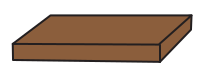
\includegraphics[width=100pt, keepaspectratio]{../figuras/licao01/ativ1_fig02a.png}
  \end{center}
  \item Considerando a divisão da barra de chocolate em 3 partes iguais, como você nomearia a quantidade de chocolate que cada amigo receberia?
\end{enumerate} %s

\subsection{Atividade}
Três pizzas inteiras, de mesmo tamanho, foram repartidas entre as crianças de uma turma. Para isso, a turma foi dividida em três grupos com quatro crianças cada. Veja como cada grupo repartiu a sua pizza.

  \begin{center}
    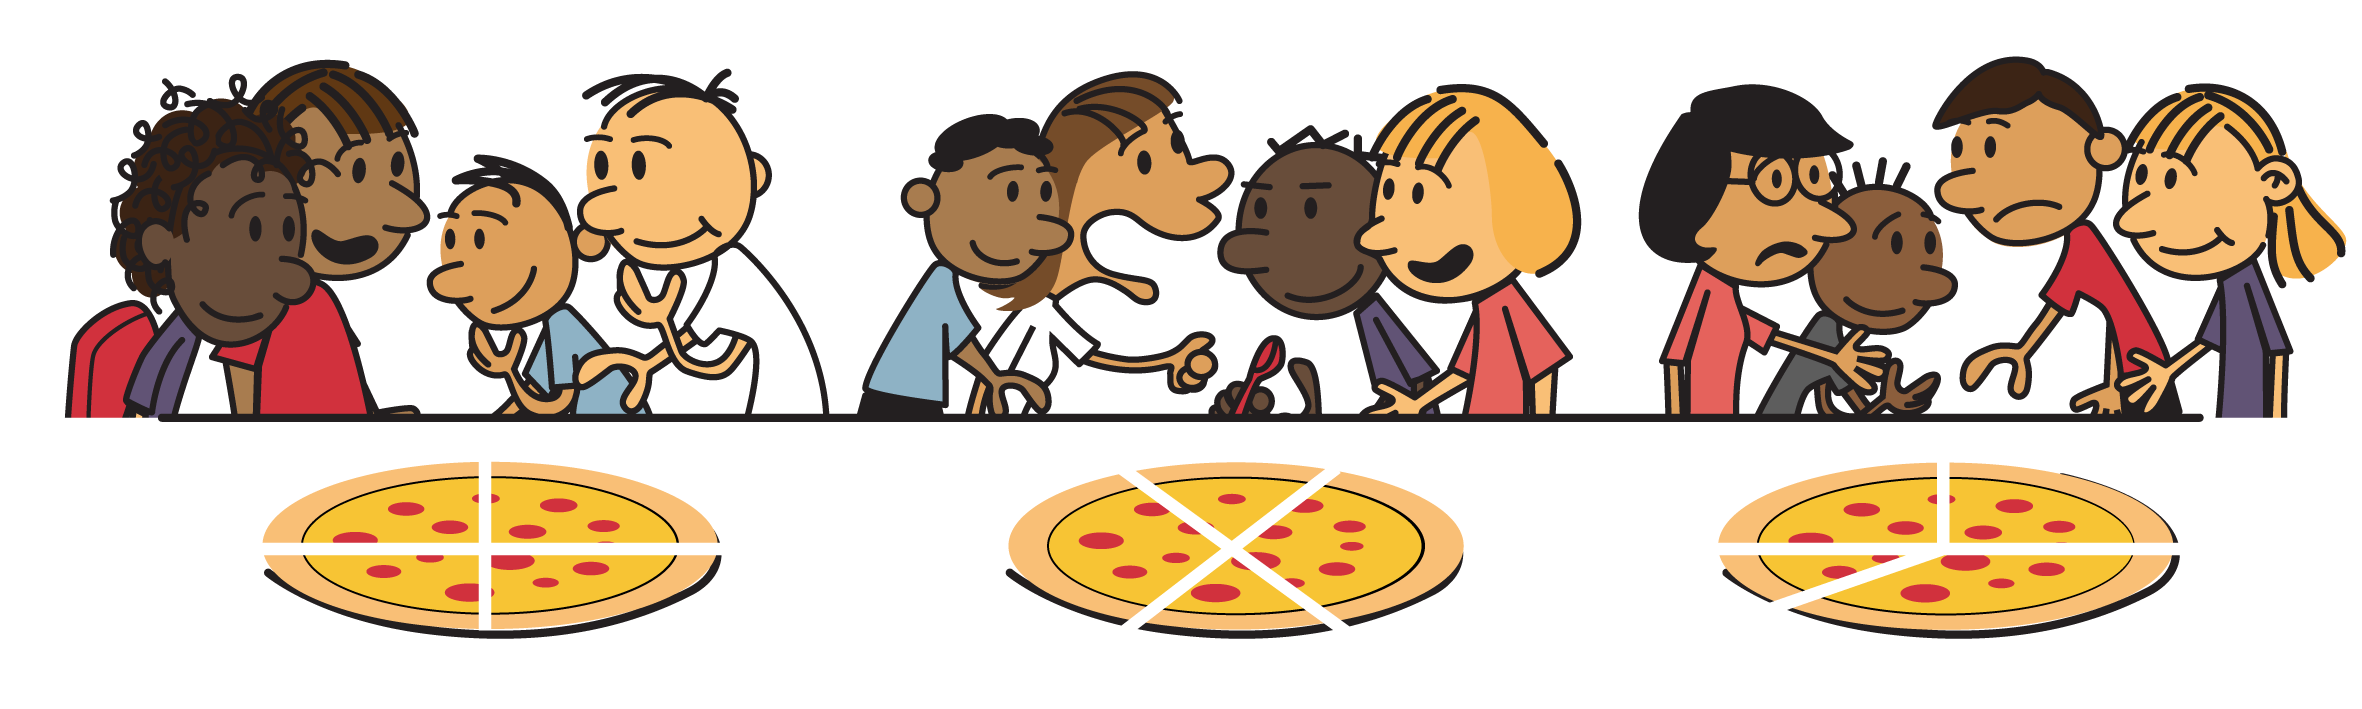
\includegraphics[width=400pt, keepaspectratio]{../figuras/licao01/ativ2_fig01.png}

    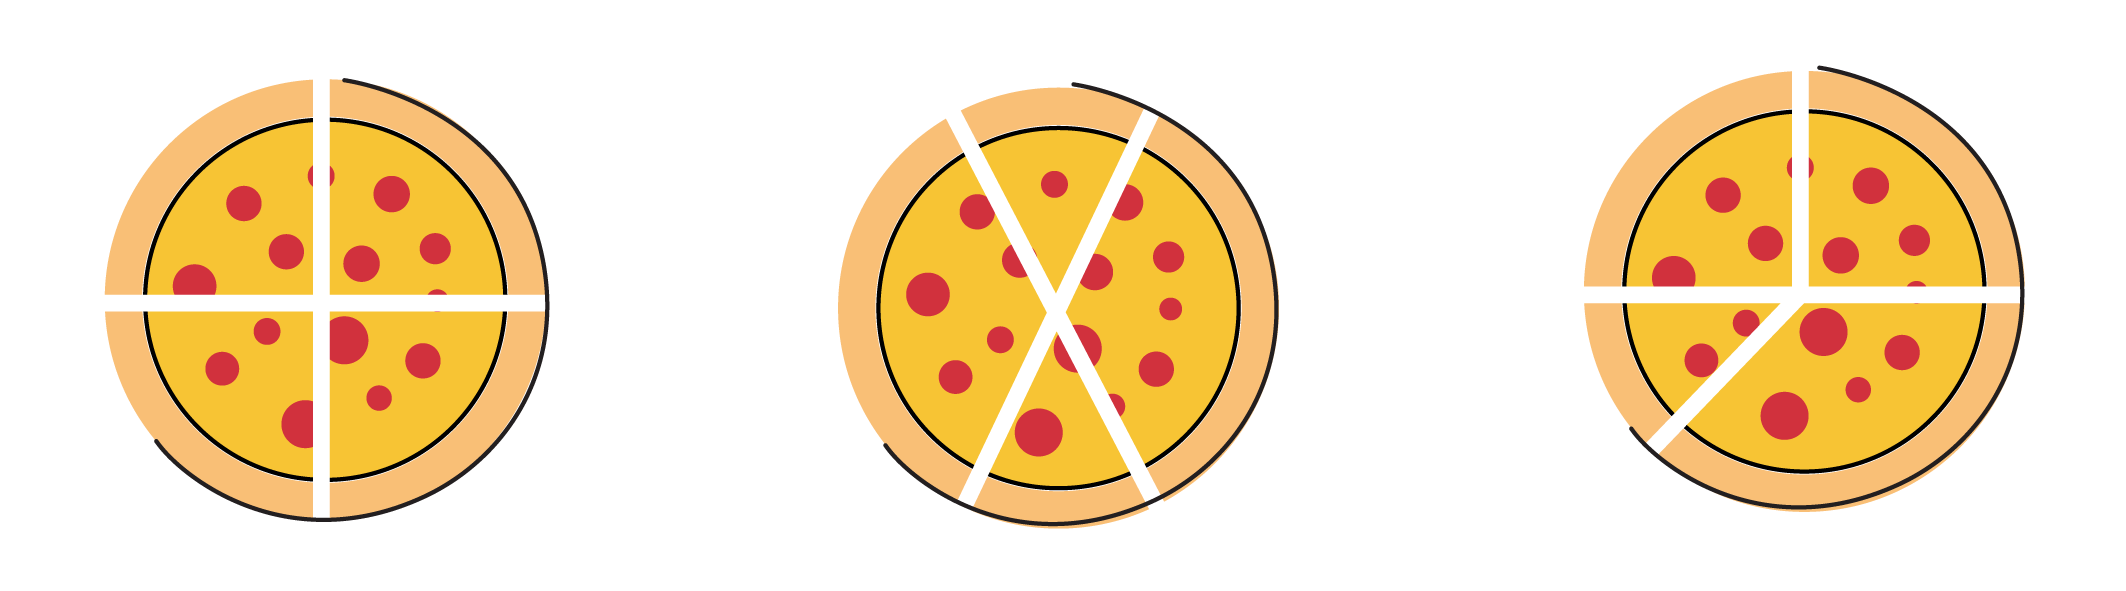
\includegraphics[width=300pt, keepaspectratio]{../figuras/licao01/ativ2_fig02.png}
  \end{center}

\begin{enumerate} [\quad a)] %d
  \item Cada um dos três grupos repartiu a sua pizza na mesma \textbf{quantidade de fatias} que os outros grupos?
  \item Dessa maneira, todas as crianças da turma receberam a mesma \textbf{quantidade de pizza}?
  \item É verdade que em algum dos grupos, as 4 crianças receberam a mesma quantidade de pizza? Se sim, em qual? Considerando a pizza inteira, como você nomearia cada uma das fatias de pizza desse grupo?
\end{enumerate} %d

\subsection{Atividade}

Alice quer enfeitar a sala de aula e pretende fazer 4 enfeites utilizando pedaços de barbante. Para isso, precisa cortar o barbante em pedaços iguais. Ajude Alice a cortar o barbante (você receberá o barbante do seu professor).

\begin{center}
    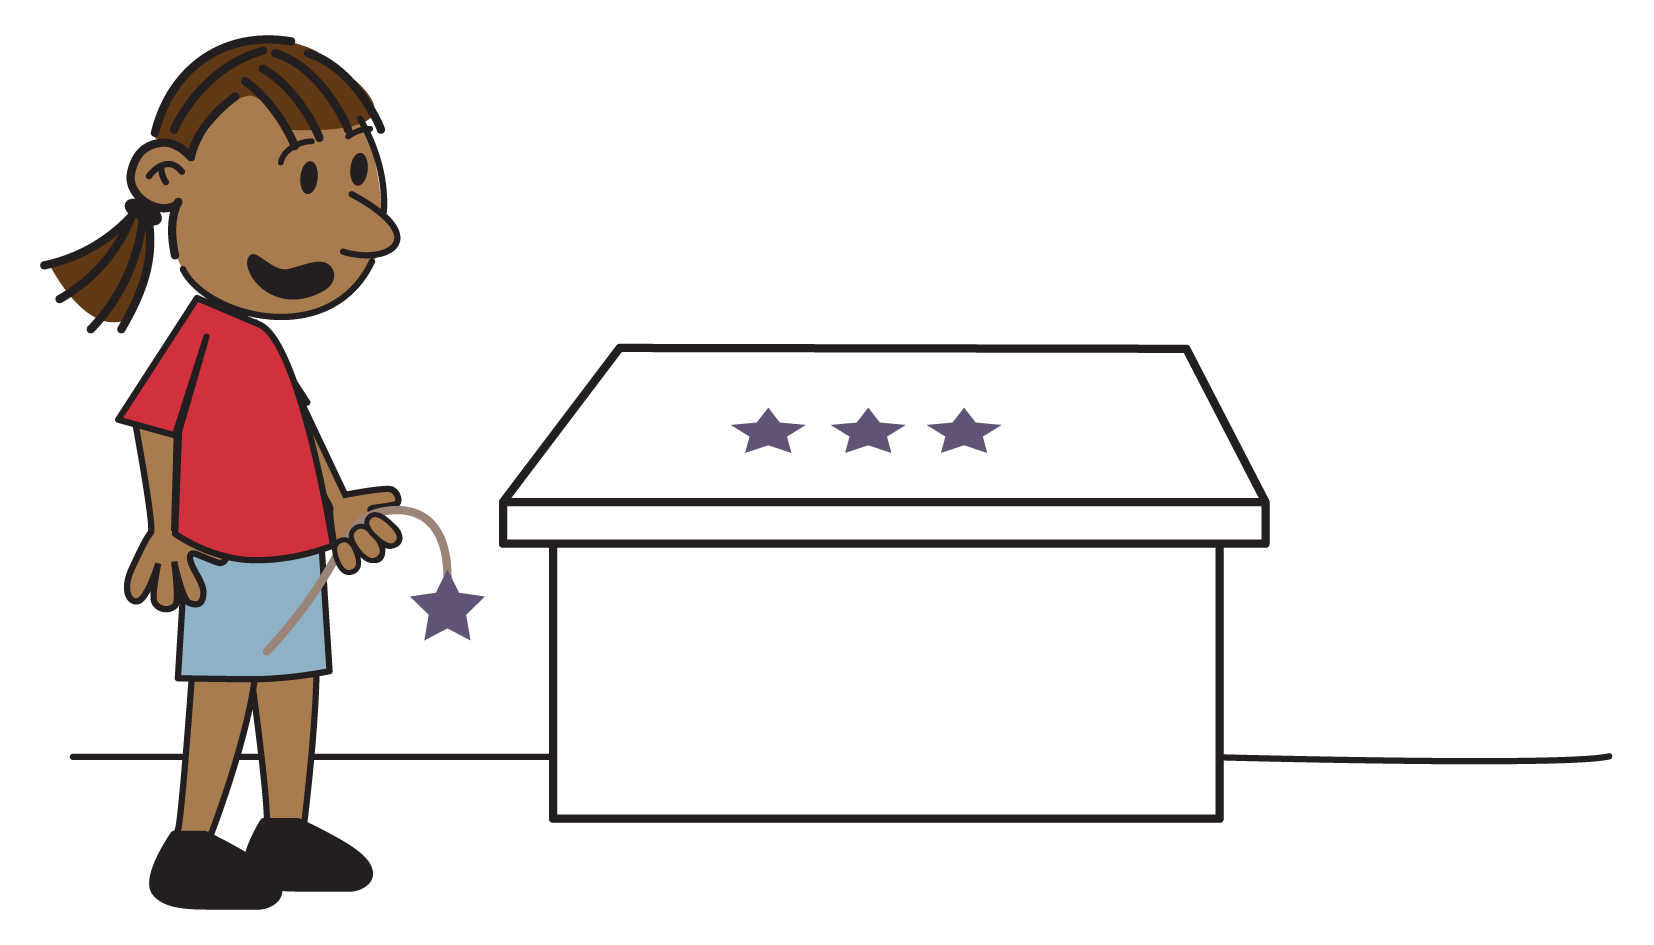
\includegraphics[width=400pt, keepaspectratio]{../figuras/licao01/ativ3_fig01.png}
  \end{center}


\section{ORGANIZANDO AS IDEIAS }

Nas atividades anteriores, a barra de chocolate, a pizza e o pedaço de barbante foram partidos \textbf{em partes com quantidades iguais}.
Em cada um dos casos, o que foi repartido é chamado \textbf{unidade}. Cada uma das partes em que essas unidades foram repartidas igualmente é uma \textbf{fração da unidade}. Assim, por exemplo, um quarto de uma pizza é uma fração da pizza e a pizza é unidade. Se a unidade for um barbante, um quarto do barbante será uma fração do barbante.

\begin{center}
    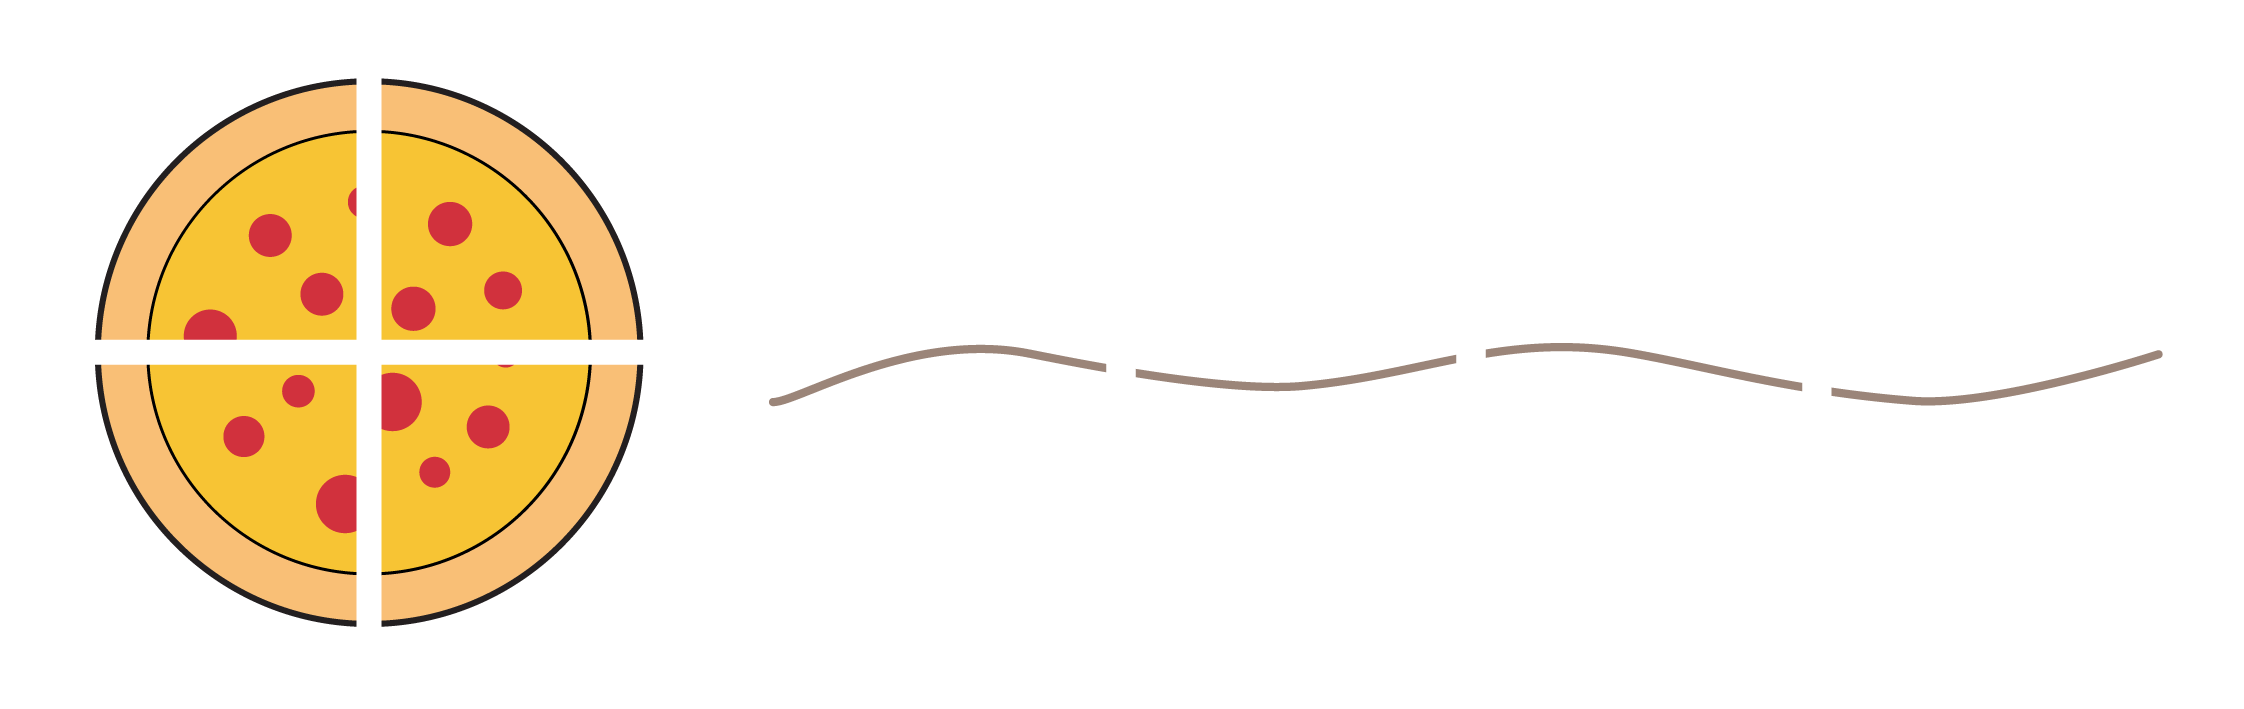
\includegraphics[width=300pt, keepaspectratio]{../figuras/licao01/orgideias_fig01.png}
  \end{center}

O nome dado à fração da unidade depende da quantidade de partes em que a unidade é dividida.
Ao dividir uma unidade qualquer em duas partes iguais, ou ao meio, cada uma das partes é chamada de \textit{um meio} ou \textit{a metade} da unidade.

Por exemplo, se uma barra de chocolate é repartida igualmente entre dois amigos, a quantidade que caberá a cada um dos amigos é \textit{um meio} da barra de chocolate (ou \textit{metade} da barra). Nesse exemplo, a unidade é a barra de chocolate.

\begin{center}
    
\includegraphics[width=400pt, keepaspectratio]{../figuras/licao01/orgideias_fig02.png}
  \end{center}

Ao dividir uma unidade em três partes iguais, cada uma das partes é chamada de \textit{um terço} ou \textit{a terça parte} da unidade.

Por exemplo, se em uma receita, é necessário acrescentar \textit{um terço} de copo de suco de laranja, isso significa que, para colocar a quantidade correta de suco na receita, é preciso repartir a quantidade de um copo de suco em três partes iguais e usar apenas uma dessas partes, que é \textit{um terço} do copo de suco. Nesse caso, a unidade é um copo de suco de laranja.

\begin{center}
    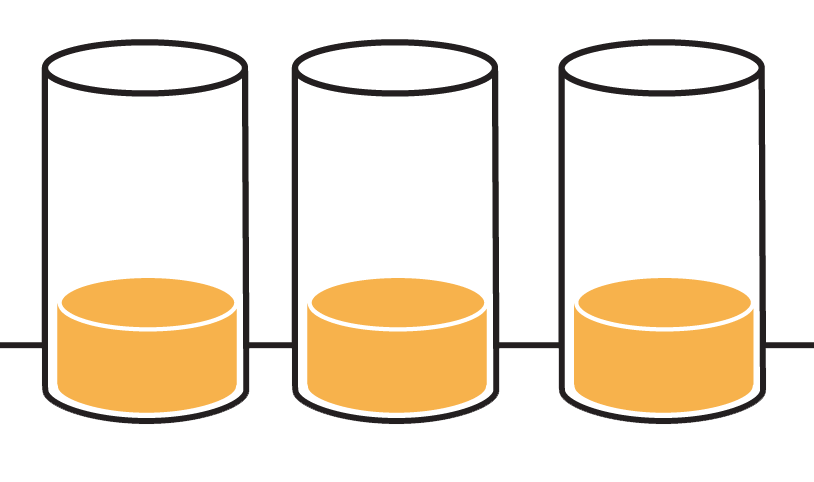
\includegraphics[width=180pt, keepaspectratio]{../figuras/licao01/orgideias_fig03a.png}
  \end{center}

Ao dividir uma unidade em quatro partes iguais, cada uma das partes é chamada de \textit{um quarto} ou \textit{quarta parte} da unidade.

Por exemplo, a parte colorida da figura é um quarto da figura. Neste caso, a figura é a unidade.

\begin{center}
    
\includegraphics[width=100pt, keepaspectratio]{../figuras/licao01/orgideias_fig04.png}
  \end{center}
Da mesma forma, ao dividir uma unidade em cinco partes iguais, cada uma das partes é chamada de \textit{um quinto} ou \textit{quinta parte} da unidade.

Por exemplo, na época do império \emph{um quinto} de todo ouro pesado nas Casas de Fundição no Brasil era pago em impostos à Coroa Portuguesa. Desta forma, a quantidade de ouro pago em impostos à Coroa Portuguesa era igual a \emph{um quinto} ou a \emph{quinta parte} do ouro pesado nas Casas de Fundição no Brasil.

\begin{center}
    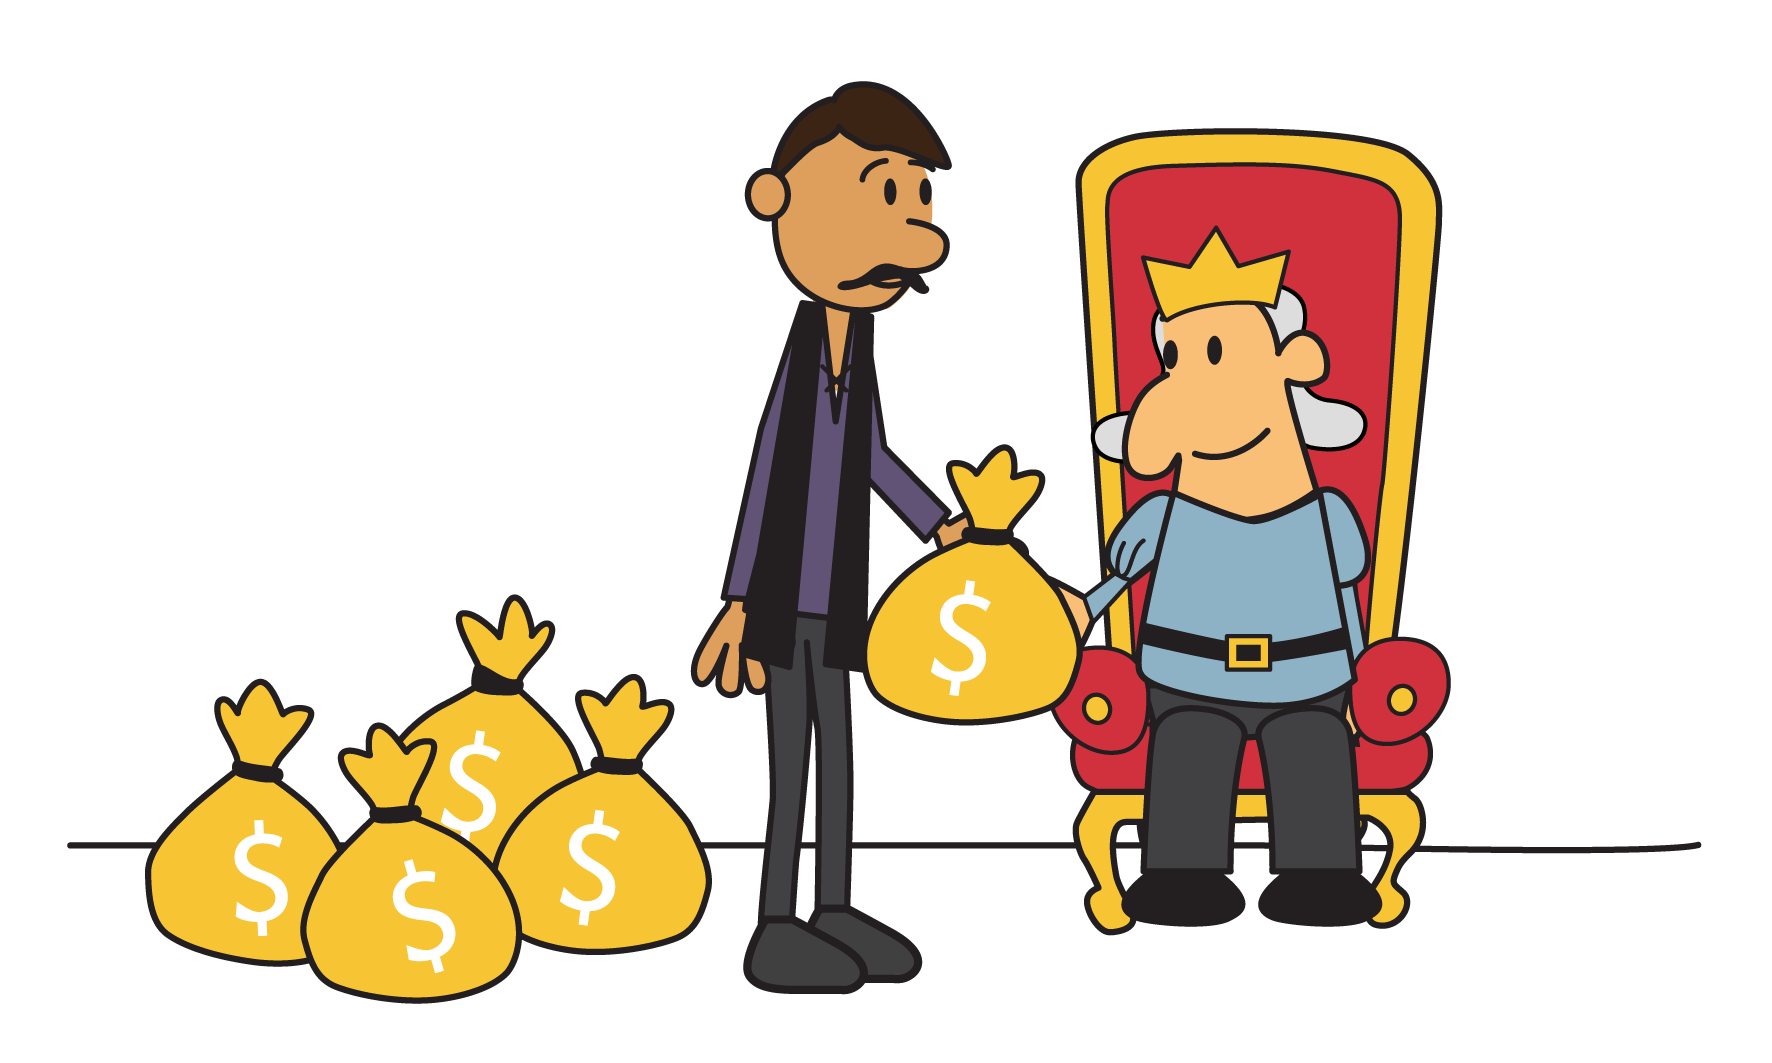
\includegraphics[width=400pt, keepaspectratio]{../figuras/licao01/orgideias_fig05.png}
  \end{center}

%   Outros exemplos aparecem no dia a dia: ``tomei meio copo de leite'' e ``gastei um terço da minha borracha''.

%   ILUSTRAÇÕES DESTA ÚLTIMA FRASE.
   
\section{MÃO NA MASSA }

\subsection{Atividade}

\begin{enumerate} [\quad a)] %s
  \item     Quais dos oito retângulos a seguir foram repartidos em {\it quartos}? \mbox{} \newline
 %\vspace{0.2cm}
\begin{center}
 \begin{tikzpicture}[scale=5]
  \draw[fill=common, fill opacity=.3] (0,0) rectangle (1,6);
  \draw[fill=common, fill opacity=.3] (1,0) rectangle (2,6);
  \draw[fill=common, fill opacity=.3] (2,0) rectangle (3,6);
  \draw[fill=common, fill opacity=.3] (3,0) rectangle (4,6);
  \draw[fill=common, fill opacity=.3] (5,0) rectangle (9,3);
  \draw[fill=common, fill opacity=.3] (5,3) rectangle (9,6);
  \draw (5,0) -- (9,3);
  \draw (5,3) -- (9,6);
  \draw[fill=common, fill opacity=.3] (10,0) rectangle (14,3);
  \draw[fill=common, fill opacity=.3] (10,3) rectangle (14,6);
  \draw (12,0) -- (12,3);
  \draw (10,4.5) -- (14,4.5);
  \draw[fill=common, fill opacity=.3] (15,0) rectangle (19,3);
  \draw[fill=common, fill opacity=.3] (15,3) rectangle (19,6);
  \draw (15,1.5) -- (19,1.5);
  \draw (15,3) -- (19,6);
\end{tikzpicture}

\vspace{0.2cm}

\begin{tikzpicture}[scale=5]
  \draw[fill=common, fill opacity=.3] (0,0) rectangle (4,1.5);
  \draw[fill=common, fill opacity=.3] (0,1.5) rectangle (4,3);
  \draw[fill=common, fill opacity=.3] (0,3) rectangle (4,4.5);
  \draw[fill=common, fill opacity=.3] (0,4.5) rectangle (4,6);
  \draw[fill=common, fill opacity=.3] (5,0) rectangle (9,3);
  \draw[fill=common, fill opacity=.3] (5,3) rectangle (9,6);
  \draw (7,0) -- (7,6);
  \draw[fill=common, fill opacity=.3] (10,0) rectangle (14,3);
  \draw[fill=common, fill opacity=.3] (10,3) rectangle (14,6);
  \draw (12,0) -- (12,3);
  \draw (10,3) -- (14,6);
  \draw[fill=common, fill opacity=.3] (15,0) rectangle (19,3);
  \draw[fill=common, fill opacity=.3] (15,3) rectangle (19,6);
  \draw (15,0) -- (19,3);
  \draw (19,3) -- (15,6);
\end{tikzpicture}
\end{center}

  \item     Desenhe um retângulo e faça uma partição desse retângulo em quatro partes que não sejam todas quartos.
\end{enumerate}

\begin{refletindo*}[breakable]{}{}
  Quando se diz que uma unidade é repartida em meios, terços, quartos, quintos, etc., a unidade foi repartida em 2, 3, 4, 5, etc., partes iguais.
  Assim como no dia a dia, neste livro o termo   {\it partes iguais}   quer dizer   {\it partes com a mesma quantidade}, mesmo que a unidade não esteja dividida em partes de mesma forma.
  Na atividade anterior, se os retângulos representassem, por exemplo, bolos, as quatro partes em que foram divididos os retângulos representariam quantidades iguais de bolo.
  Em alguns retângulos as partes não têm a mesma forma.
  Os dois quadrinhos a seguir mostram exemplos curiosos em que as partes iguais podem ser surpreendentes.

  \noindent\begin{tabular}{ll}
    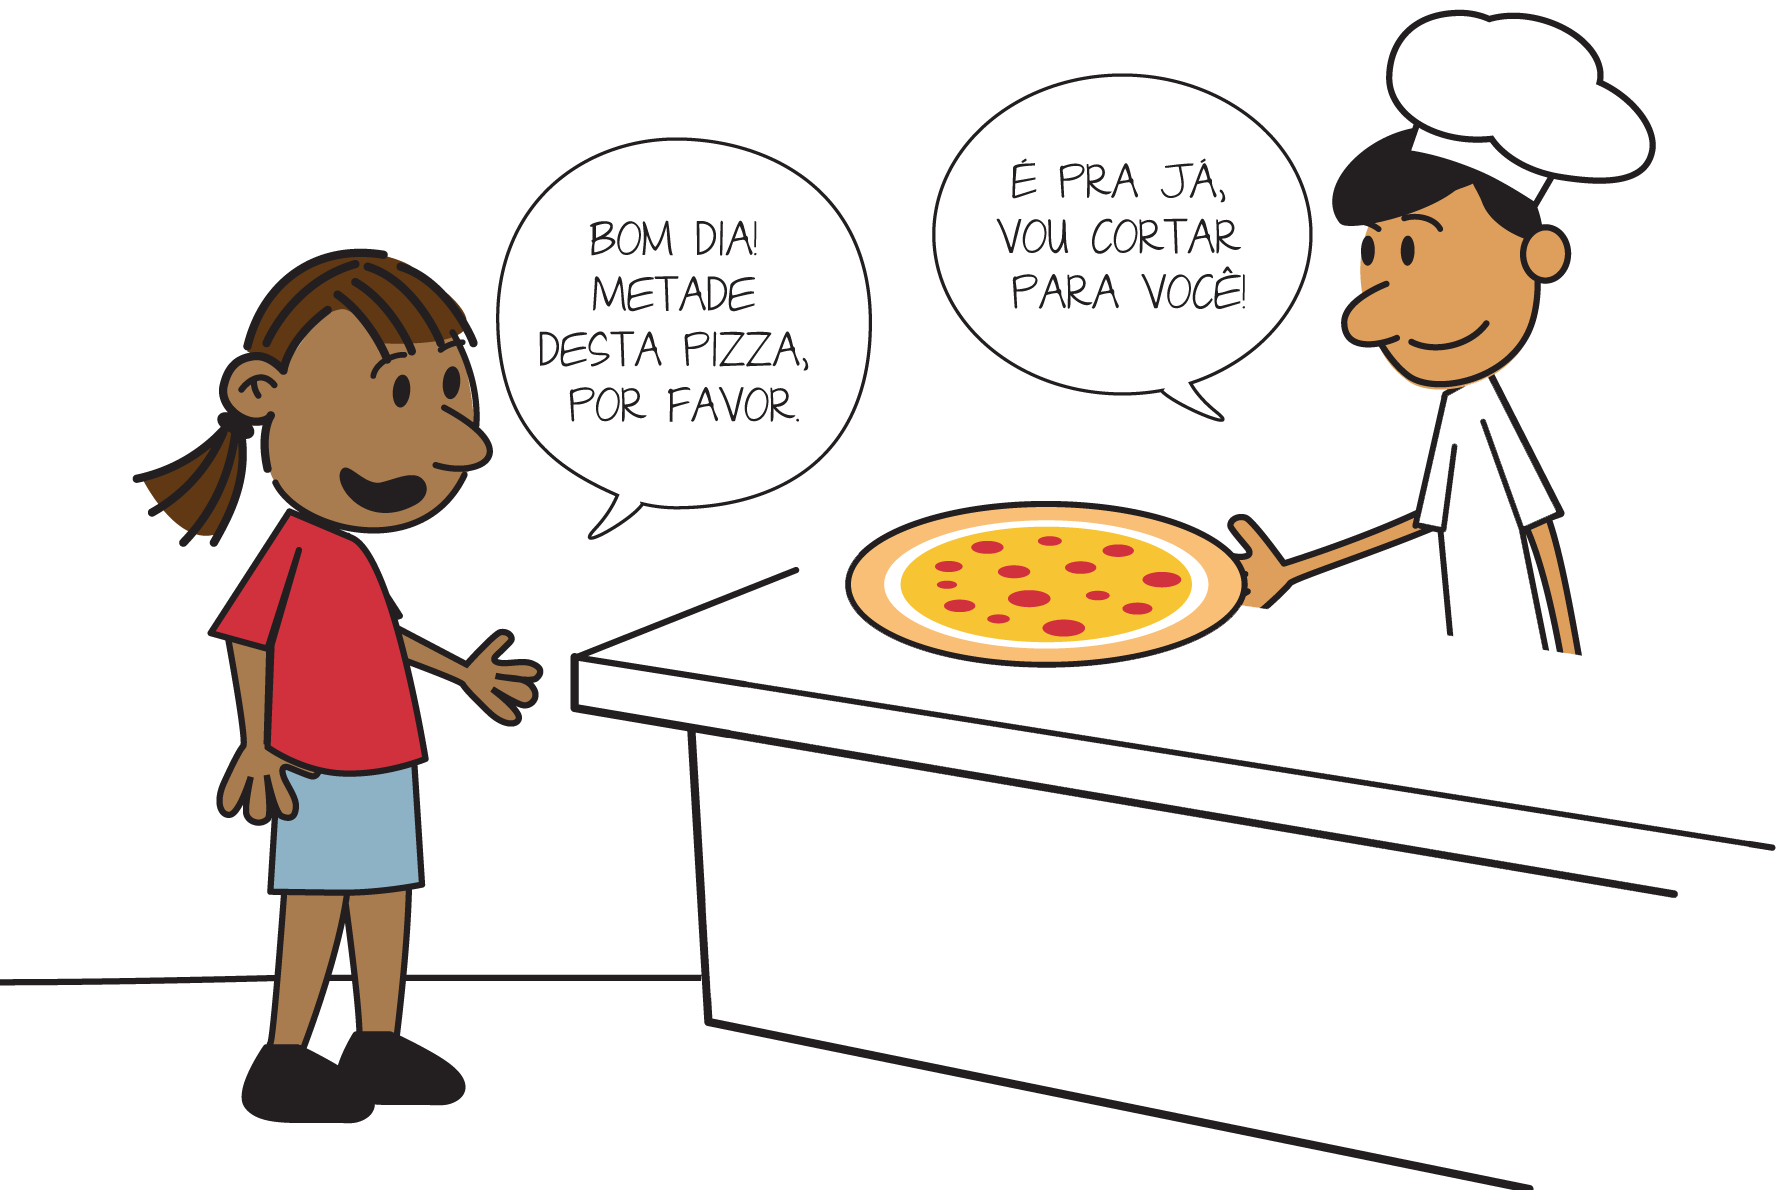
\includegraphics[width=220pt, keepaspectratio]{../figuras/licao01/reflet_fig01.png} & 
\includegraphics[width=180pt, keepaspectratio]{../figuras/licao01/reflet_fig02.png}

  \end{tabular}
\vspace{.5cm}
  \hline
  \vspace{.5cm}

  \noindent  \noindent\begin{tabular}{ll}
    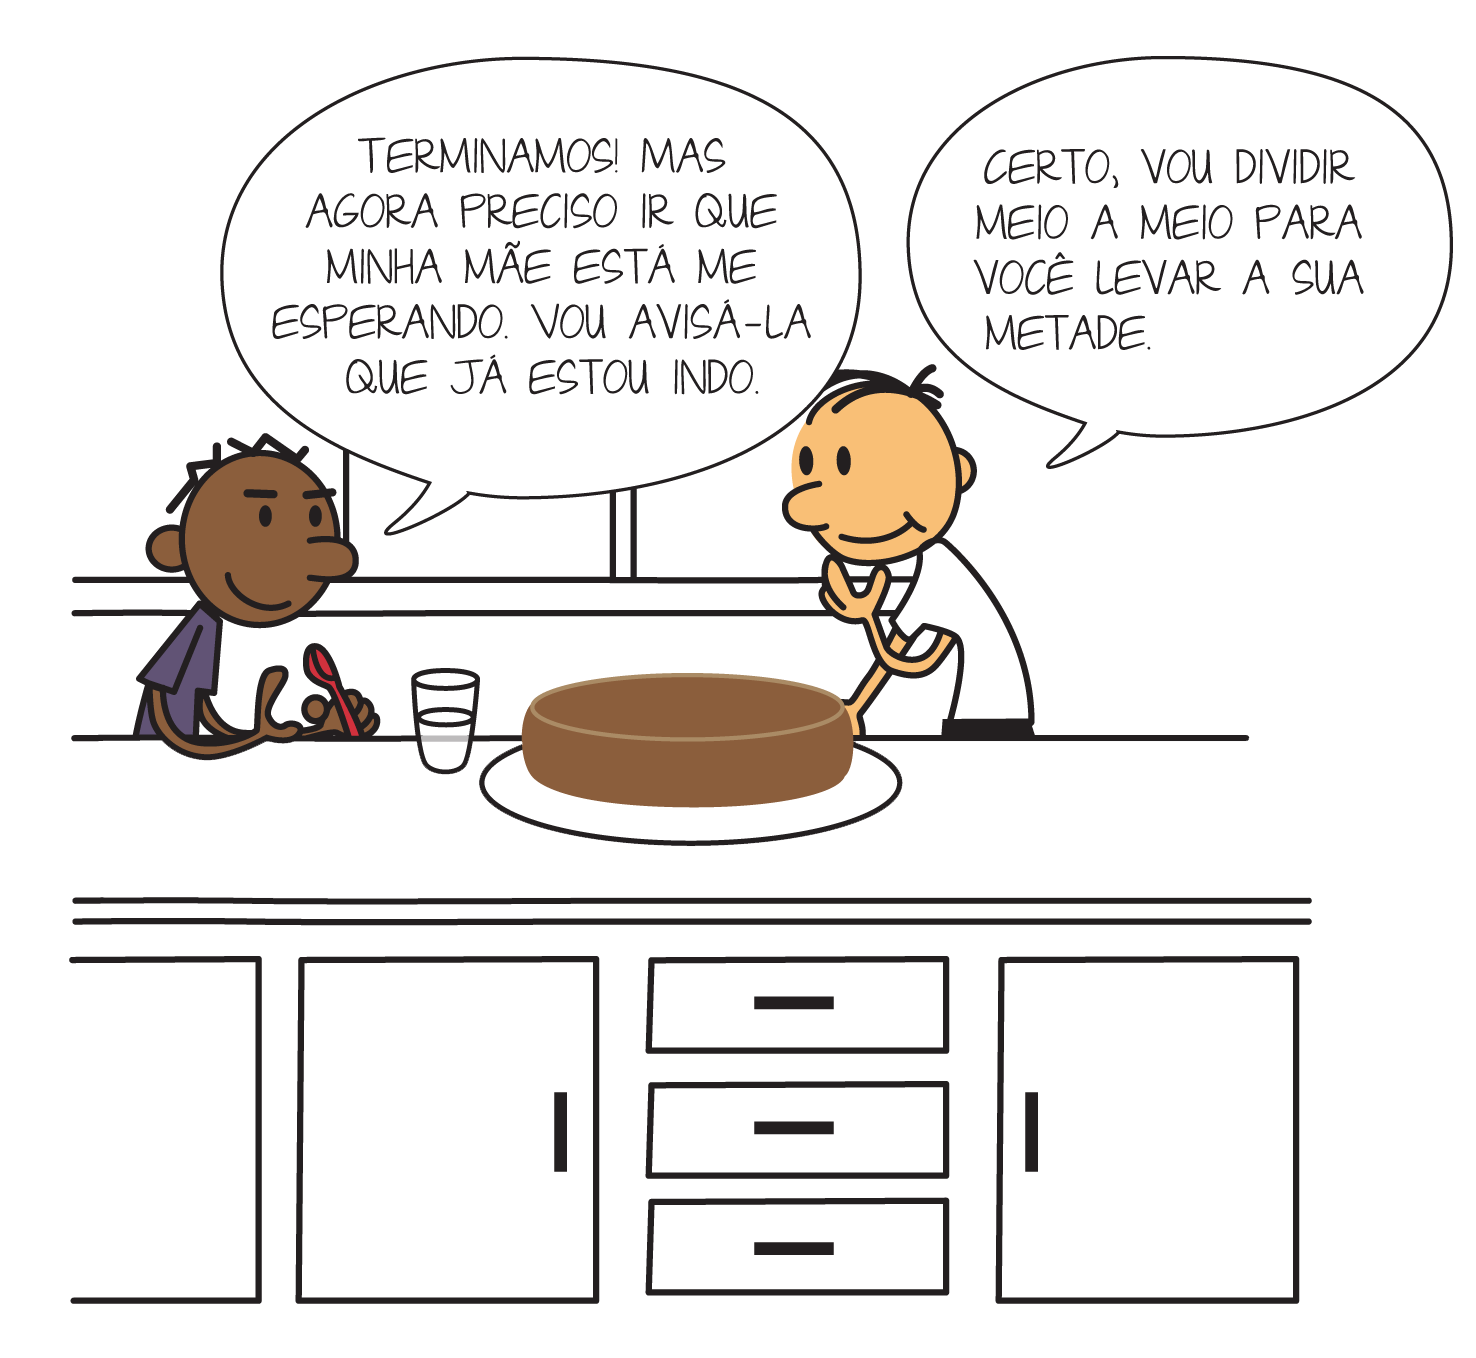
\includegraphics[width=180pt, keepaspectratio]{../figuras/licao01/reflet_fig03.png}   & 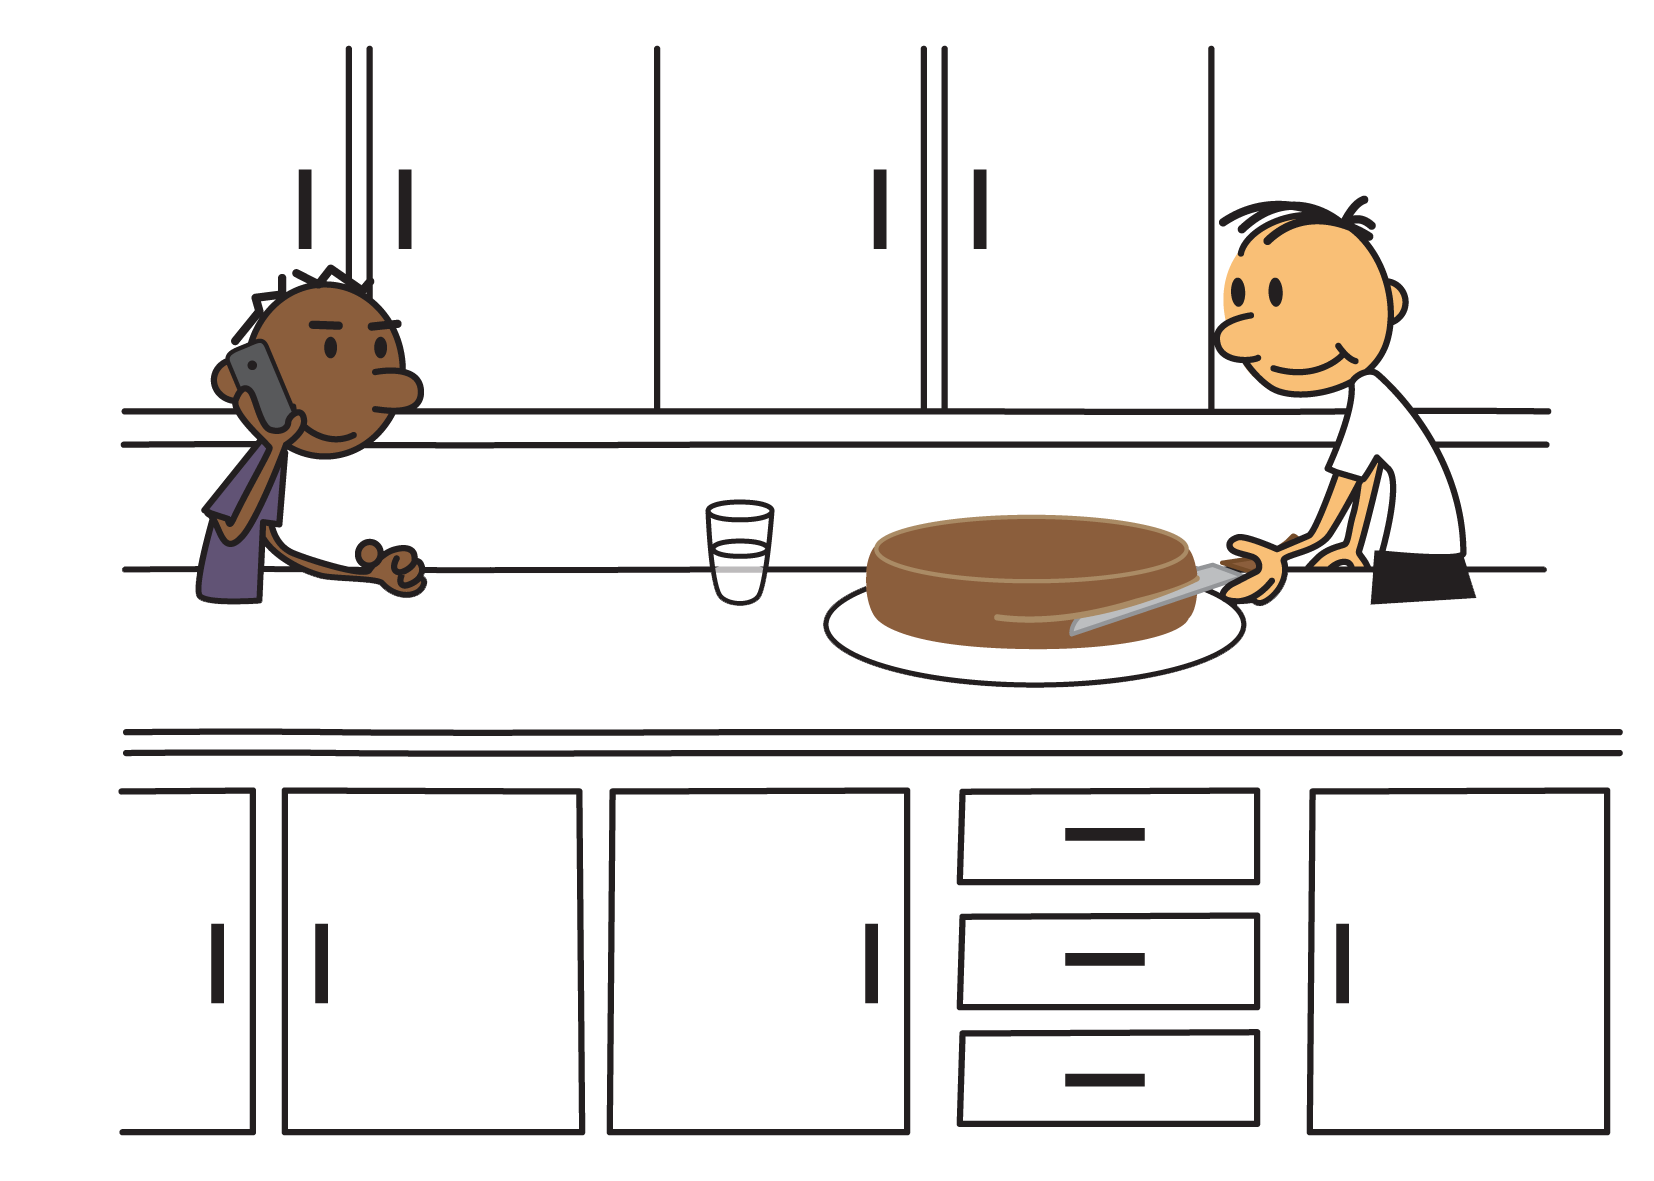
\includegraphics[width=200pt, keepaspectratio]{../figuras/licao01/reflet_fig04.png}
  \end{tabular}




\end{refletindo*}


\subsection{Atividade}

Em cinco das figuras a seguir, a parte em vermelho é um terço da figura. Identifique essas figuras.

\begin{center}
\begin{longtable}{ccc}
a)
\parbox[t][3cm][c]{5cm}{
  \begin{tikzpicture}[scale=0.7]
    \draw[very thick, attention] (90:2 cm)  -- (210:2 cm);
    \draw[very thick, attention] (330:2 cm) -- (90:2 cm);
    \draw[very thick, common] (210:2 cm)  -- (330:2 cm);
  \end{tikzpicture}
}
& \quad \quad  &

b)
\parbox[t][3cm][c]{5cm}{
\begin{tikzpicture}[scale=6]
  \filldraw[fill=common, fill opacity=.3, draw=black] (0,0) -- (0.5,0.5) -- (3.5,0.5) -- (3.5,2.5) -- (4,3) -- (4,0)--cycle;
  \fill[attention] (0,0) -- (0.5,0.5) -- (0.5,2.5) -- (3.5,2.5) -- (4,3) -- (0,3)--cycle;
  \draw (0,0) rectangle (4,3);
  \draw (0.5,0.5) rectangle (3.5,2.5);
\end{tikzpicture}
}
\\

c)
\parbox[t][3cm][c]{5cm}{
\begin{tikzpicture}[scale=4]
  \draw[very thick, common] (0,3) -- (3,0);
  \draw[very thick, attention] (3,0) -- (6,3);
  \draw[very thick, common] (6,3) -- (9,0);
\end{tikzpicture}
}
& &

d)
\parbox[t][3cm][c]{5cm}{
\begin{tikzpicture}[scale=0.7]
  \draw[very thick, common] (90:2 cm)  -- (210:2 cm);
  \draw[very thick, attention] (210:2 cm)  -- (330:2 cm);
  \draw[very thick, common] (330:2 cm) -- (90:2 cm);
\end{tikzpicture}
    }\\

e)
\parbox[t][3cm][c]{5cm}{

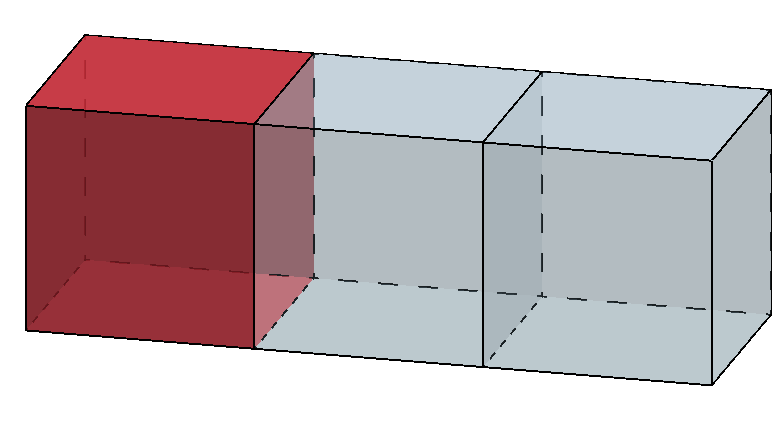
\includegraphics[scale=.6]{..figuras/licao01/paralelepipedo_tercos.png}
}
%   \begin{tikzpicture}%[scale=60]
%   \tikzset{
%   annotated cuboid/.pic={
%     \tikzset{%
%       every edge quotes/.append style={midway, auto},
%       /cuboid/.cd,
%       #1
%     }
%     \draw [every edge/.append style={pic actions, densely dashed, opacity=0}, pic actions]
%     (0,0,0) coordinate (o) -- ++(-\cubescale*\cubex,0,0) coordinate (a) -- ++(0,-\cubescale*\cubey,0) coordinate (b) edge coordinate [pos=1] (g) ++(0,0,-\cubescale*\cubez)  -- ++(\cubescale*\cubex,0,0) coordinate (c) -- cycle
%     (o) -- ++(0,0,-\cubescale*\cubez) coordinate (d) -- ++(0,-\cubescale*\cubey,0) coordinate (e) edge (g) -- (c) -- cycle
%     (o) -- (a) -- ++(0,0,-\cubescale*\cubez) coordinate (f) edge (g) -- (d) -- cycle;
%  },
%   /cuboid/.search also={/tikz},
%   /cuboid/.cd,
%   width/.store in=\cubex,
%   height/.store in=\cubey,
%   depth/.store in=\cubez,
%   units/.store in=\cubeunits,
%   scale/.store in=\cubescale,
%   width=100,
%   height=100,
%   depth=100,
%   units=cm,
%   scale=.1,
% }
%
%     \pic [fill=attention, fill opacity=.8] at (50,0) {annotated cuboid={width=100, height=100, depth=14}};
%     \pic [fill=common, fill opacity=.3] at (60,0) {annotated cuboid={width=100, height=100, depth=14}};
%     \pic [fill=common, fill opacity=.3] at (70,0) {annotated cuboid={width=100, height=100, depth=14}};
%     \end{tikzpicture}
% }
&&

f)
\parbox[t][3cm][c]{5cm}{
\begin{tikzpicture}[scale=0.7]
  \fill[attention] (0,0) -- (60:2 cm) -- (120:2 cm) -- (180:2 cm) -- (0,0);
  \filldraw[fill=common, draw=black, fill opacity=.3] (0,0) -- (60:2 cm) -- (0:2 cm) -- (300:2 cm) -- (240:2 cm) -- (180:2 cm) -- (0,0);
  \foreach \x in {0,60,...,300}{
      \draw (\x:2 cm)  -- (\x + 60:2 cm);}
      \draw (0,0)  -- (60:2 cm);
      \draw (0,0)  -- (180:2 cm);
      \draw (0,0)  -- (300:2 cm);
\end{tikzpicture}
}
\\

g)
\parbox[t][3cm][c]{5cm}{
  \begin{tikzpicture}[scale=4]
    \draw[very thick, attention] (0,3) -- (3,0);
    \draw[very thick, attention] (3,0) -- (6,3);
    \draw[very thick, common] (6,3) -- (9,0);
  \end{tikzpicture}
}
&&
h)
\parbox[t][3cm][c]{5cm}{
\begin{tikzpicture}[scale=3]
    \draw[fill=common, fill opacity=.3] (0,0) rectangle (3,1);
    \draw[fill=attention] (3,0) rectangle (6,1);
    \draw[fill=common, fill opacity=.3] (6,0) rectangle (9,1);
\end{tikzpicture}
}
\\

i)
\parbox[t][3cm][c]{5cm}{
\begin{tikzpicture}[scale=3]
    \draw[fill=common, fill opacity=.3] (0,0) rectangle (2,1);
    \draw[fill=attention] (2,0) rectangle (6,1);
    \draw[fill=common, fill opacity=.3] (6,0) rectangle (9,1);
\end{tikzpicture}
}&&
j)
\parbox[t][3cm][c]{5cm}{
\begin{tikzpicture}[scale=0.7]
 \fill[attention] (162:2 cm) -- (234:2 cm) -- (306: 2 cm) -- (378: 2cm) -- (0,0) -- cycle;
 \filldraw[fill=common, draw=black, fill opacity=.3] (162:2 cm) -- (0,0) -- (378: 2cm) -- (90: 2cm) -- cycle;
  \foreach \x in {90,162,...,378}{
 \draw (\x: 2cm) -- (\x + 72: 2cm);
 \draw (0,0) -- (\x:2cm);}
\end{tikzpicture}
}
\end{longtable}
\end{center}

\subsection{Atividade}

Observe a tabela a seguir. Em cada linha, a primeira coluna, mais à esquerda, exibe figuras que são frações de uma unidade. A coluna do meio indica essas frações. Complete a tabela, fazendo na terceira coluna de cada linha, um desenho da unidade correspondente.

\begin{center}
  \begin{tabular}{|m{0.3\linewidth}|m{0.3\linewidth}|m{0.3\linewidth}|}
  \hline
\centering Parte da unidade & \centering Fração da unidade  & \quad\quad\quad Unidade  \\
\hline \hline
\centering \begin{tikzpicture}[scale=2]
 \draw [fill=common, fill opacity=.3] (0,0) arc (0:90:3) -- (-3,0) -- cycle;
\end{tikzpicture}
&\centering \parbox[c][1.2cm][c]{0.01cm}{  } metade  &  \\
    \hline
\centering\begin{tikzpicture}[scale=2]
\draw [fill=common, fill opacity=.3] (0,0) arc (0:90:3) -- (-3,0) -- cycle;
\end{tikzpicture}        &\parbox[c][1.2cm][c]{0.01cm}{  } \centering   um terço  &  \\
    \hline
\centering \begin{tikzpicture}[scale=2]
\draw [fill=common, fill opacity=.3] (0,0) arc (0:90:3) -- (-3,0) -- cycle;
\end{tikzpicture}        & \centering \parbox[c][1.2cm][c]{0.01cm}{  } um quarto  &  \\
    \hline
\centering \begin{tikzpicture}[scale=2]
\draw [fill=common, fill opacity=.3] (0,0) rectangle (3,3);
\end{tikzpicture}
  & \centering \parbox[c][1.2cm][c]{0.01cm}{  } metade  &  \\
    \hline
\centering \begin{tikzpicture}[scale=2]
\draw [fill=common, fill opacity=.3] (0,0) rectangle (3,3);
\end{tikzpicture}
  & \centering \parbox[c][1.2cm][c]{0.01cm}{  } um terço  &  \\
    \hline
\centering \begin{tikzpicture}[scale=2]
\draw [fill=common, fill opacity=.3] (0,0) rectangle (3,3);
\end{tikzpicture}
 & \centering \parbox[c][1.2cm][c]{0.01cm}{  } um quarto  &  \\
    \hline
\centering \begin{tikzpicture}[scale=2]
\draw  (0,0) -- (3,3);
\end{tikzpicture}
  & \centering \parbox[c][1.2cm][c]{0.01cm}{  } metade  &  \\
    \hline
\centering \begin{tikzpicture}[scale=2]
\draw  (0,0) -- (3,3);
\end{tikzpicture}
  & \centering \parbox[c][1.2cm][c]{0.01cm}{  } um terço  &  \\
    \hline
\centering \begin{tikzpicture}[scale=2]
\draw  (0,0) -- (3,3);
\end{tikzpicture}
  & \centering \parbox[c][1.2cm][c]{0.01cm}{  } um quarto  &  \\
    \hline
\centering \begin{tikzpicture}[scale=2]
\draw [fill=common, fill opacity=.3] (0,0) -- (3,0) -- (-1.5,1.5) -- cycle;
\end{tikzpicture}  & \centering \parbox[c][1.2cm][c]{0.01cm}{  } metade  &  \\
    \hline
\centering \begin{tikzpicture}[scale=2]
\draw [fill=common, fill opacity=.3] (0,0) -- (3,0) -- (-1.5,1.5) -- cycle;
\end{tikzpicture}  & \centering \parbox[c][1.2cm][c]{0.01cm}{  } um terço  &  \\
    \hline
\centering \begin{tikzpicture}[scale=2]
\draw [fill=common, fill opacity=.3] (0,0) -- (3,0) -- (-1.5,1.5) -- cycle;
\end{tikzpicture}  & \centering \parbox[c][1.2cm][c]{0.01cm}{  } um quarto  &  \\
    \hline
  \end{tabular}
\end{center}

\pagebreak
\subsection{Atividade}

\begin{enumerate} [\quad a)] %s
  \item     Pinte metade do quadrado a seguir.

  \begin{center}
 \begin{tikzpicture}[x=1mm,y=1mm, scale=.7]  \draw[fill=common, fill opacity=.3] (0,0) rectangle (20,20);  \end{tikzpicture}
  \end{center}

  \item     Pinte um quarto do quadrado a seguir.

  \begin{center}
 \begin{tikzpicture}[x=1mm,y=1mm, scale=.7]  \draw[fill=common, fill opacity=.3] (0,0) rectangle (20,20);  \end{tikzpicture}
  \end{center}

  \item     Pinte um oitavo do quadrado a seguir.

  \begin{center}
 \begin{tikzpicture}[x=1mm,y=1mm, scale=.7]  \draw[fill=common, fill opacity=.3] (0,0) rectangle (20,20);  \end{tikzpicture}
  \end{center}
  \item     Observando os quadrados pintados nos itens anteriores, qual é a maior das frações do quadrado: metade, quarto ou oitavo?
\end{enumerate} %s


\subsection{Atividade}

\begin{enumerate} [a)] %d
  \item     Pinte metade da figura.
\begin{center}
  \begin{tikzpicture}[x=1cm,y=1cm, scale=0.5]
  \draw[fill=common, fill opacity=.3] (3.,5.) -- (3.,3.) -- (4.7,2.) -- (6.46,3.) -- (8.2,2.) -- (9.9,3.) -- (9.9,5.) -- (8.2,6.)       -- (6.46,5.) -- (4.73,6.) -- cycle;
  \end{tikzpicture}
\end{center}

  \item     Pinte metade da figura de forma diferente da do item anterior.
\begin{center}
  \begin{tikzpicture}[x=1cm,y=1cm, scale=0.5]
  \draw[fill=common, fill opacity=.3] (3.,5.) -- (3.,3.) -- (4.7,2.) -- (6.46,3.) -- (8.2,2.) -- (9.9,3.) -- (9.9,5.) -- (8.2,6.)       -- (6.46,5.) -- (4.73,6.) -- cycle;
  \end{tikzpicture}
\end{center}

  \item     Pinte a metade da figura de forma diferente das dos dois itens anteriores.
\begin{center}
  \begin{tikzpicture}[x=1cm,y=1cm, scale=0.5]
  \draw[fill=common, fill opacity=.3] (3.,5.) -- (3.,3.) -- (4.7,2.) -- (6.46,3.) -- (8.2,2.) -- (9.9,3.) -- (9.9,5.) -- (8.2,6.)       -- (6.46,5.) -- (4.73,6.) -- cycle;
  \end{tikzpicture}
\end{center}


\end{enumerate} %d


\subsection{Atividade}

Identifique as figuras em que a parte pintada de vermelho é a metade da figura.

\begin{center}
  \begin{tabular}{ccccc}
%retângulos

\begin{tikzpicture}[scale=5]
 \draw[fill=attention] (0,0) rectangle (3,2);
 \draw[fill=common, fill opacity=.3] (3,0) rectangle (6,2);
 \node at (3,-1) {Figura 1};
\end{tikzpicture}
&
\quad \quad \quad
&
\begin{tikzpicture}[scale=5]
 \draw[fill=common, fill opacity=.3] (0,0) rectangle (3,2);
 \draw (1,0) -- (1,2);
 \draw (1.5,0) -- (1.5,2);
 \draw (2.2,0) -- (2.2,2);
 \draw[fill=attention] (3,0) rectangle (6,2);
 \node at (3,-1) {Figura 2};
\end{tikzpicture}
&
\quad \quad \quad
&

\begin{tikzpicture}[scale=5]
 \draw[fill=common, fill opacity=.3] (0,0) rectangle (3,2);
 \draw[fill=common, fill opacity=.3] (3,0) rectangle (6,2);
 \node at (3,-1) {Figura 3};
 \filldraw[fill=attention, draw=black] (0,2) rectangle (6,1.2);
 \end{tikzpicture}
\\
 % círculos

\begin{tikzpicture}[scale=5]
  \filldraw[fill=attention, draw=black] (0,-2) arc (-90:90: 2);
  \draw (0, 2) -- (0, -2);
  \draw[fill=common, fill opacity=.3] (0,2) arc (90:270:2);
  \node at (0,-3) {Figura 4};
\end{tikzpicture}
&&

\begin{tikzpicture}[scale=5]
 \filldraw[fill=attention, draw=black] (45:2) arc (45:225:2);
 \draw[fill=common, fill opacity=.3] (225:2) arc (225:405:2);
 \node at (0,-3) {Figura 5};
 \draw (0,0) -- (0,-2);
 \draw (0,0) -- (-30:2);
 \draw (225:2) -- (45:2);
 \end{tikzpicture}

 &&
 \begin{tikzpicture}[scale=5]
 \draw[fill=common, fill opacity=.3] (0,0) circle (2);
 \filldraw[fill=attention, draw=black] (0,0) -- (2,0) arc (0:90:2) -- cycle;
 \filldraw[fill=attention, draw=black] (0,0) -- (-2,0) arc (180:270: 2) -- cycle;
 \node at (0,-3) {Figura 6};
\end{tikzpicture}
\\
% hexágonos

\begin{tikzpicture}[scale=5]
 \filldraw[fill=common, fill opacity=.3] (60:2) -- (120:2) -- (180:2) -- (240:2) -- (300:2) --cycle;
 \filldraw[fill=attention, draw=black] (2,0) -- (60:2) -- (300:2) --cycle;
 \node at (0,-3) {Figura 7};
\end{tikzpicture}
& &

\begin{tikzpicture}[scale=5]
  \fill[attention] (60:2) -- (120:2) -- (180:2) -- (240:2) --cycle;
\filldraw[fill=common, fill opacity=.3] (60:2) -- (240:2) -- (300:2) -- (0:2) --cycle;
  \draw (60:2) -- (0,0) -- (240:2);
  \draw (2,0) -- (0,0) -- (300:2) (0,-3) node{Figura 8};
\end{tikzpicture}
&&

\begin{tikzpicture}[scale=5]
  \filldraw[fill=attention] (0:2) -- (60:2) -- (0:0) --cycle;
  \filldraw[fill=attention] (120:2) -- (180:2) -- (0:0) --cycle;
  \filldraw[fill=attention] (240:2) -- (300:2) -- (0:0) --cycle;
  \filldraw[fill=common, fill opacity=.3] (0,0) -- (60:2) -- (120:2)--cycle;
  \filldraw[fill=common, fill opacity=.3] (0,0) -- (0:2) -- (300:2)--cycle;
  \filldraw[fill=common, fill opacity=.3] (0,0) -- (180:2) -- (240:2)--cycle;
  \node at (0,-3) {Figura 9};
\end{tikzpicture}
\\
%círculo

\begin{tikzpicture}[scale=5]
 \draw[fill=attention] (0:2) arc (0:270:2) -- (0,0) -- cycle;
 \draw[fill=common, fill opacity=.3] (270:2) arc (270:360:2) -- (0,0) -- cycle;
 \draw (0,0) -- (0,-2);
 \draw (0,0) -- (2,0)  (0,-3) node{Figura 10};
 \end{tikzpicture}
&&
%hexágonos

\begin{tikzpicture}[scale=5]
  \filldraw[fill=attention] (120:2) -- (180:2) -- (240:2) -- cycle;
  \filldraw[fill=attention] (240:2) -- (300:2) -- (60:2) -- cycle;
  \draw[fill=common, fill opacity=.3] (60:2) -- (120:2) -- (240:2) -- cycle;
  \draw[fill=common, fill opacity=.3] (0:2) -- (300:2) -- (60:2) -- cycle;
  \node at (0,-3) {Figura 11};
\end{tikzpicture}
&&
%retângulo
\begin{tikzpicture}[scale=5]
 \draw[fill=common, fill opacity=.3] (0,-1) rectangle (6,1);
 \filldraw[fill=attention, draw=black] (1,-1) rectangle (4,1);
 \node at (3,-2) {Figura 12};
 \end{tikzpicture}

\end{tabular}
\end{center}


\subsection{Atividade}


Usando os Círculos de Frações que você receberá do seu professor (há encarte para reprodução no final do livro), responda:

\begin{center}

 \begin{tabular}{ccccccccc}

 
\begin{tikzpicture}
\fill[black] (0,0) circle (10);
 \end{tikzpicture}
& \parbox[t][.6cm][c]{1cm}{ }\quad&
 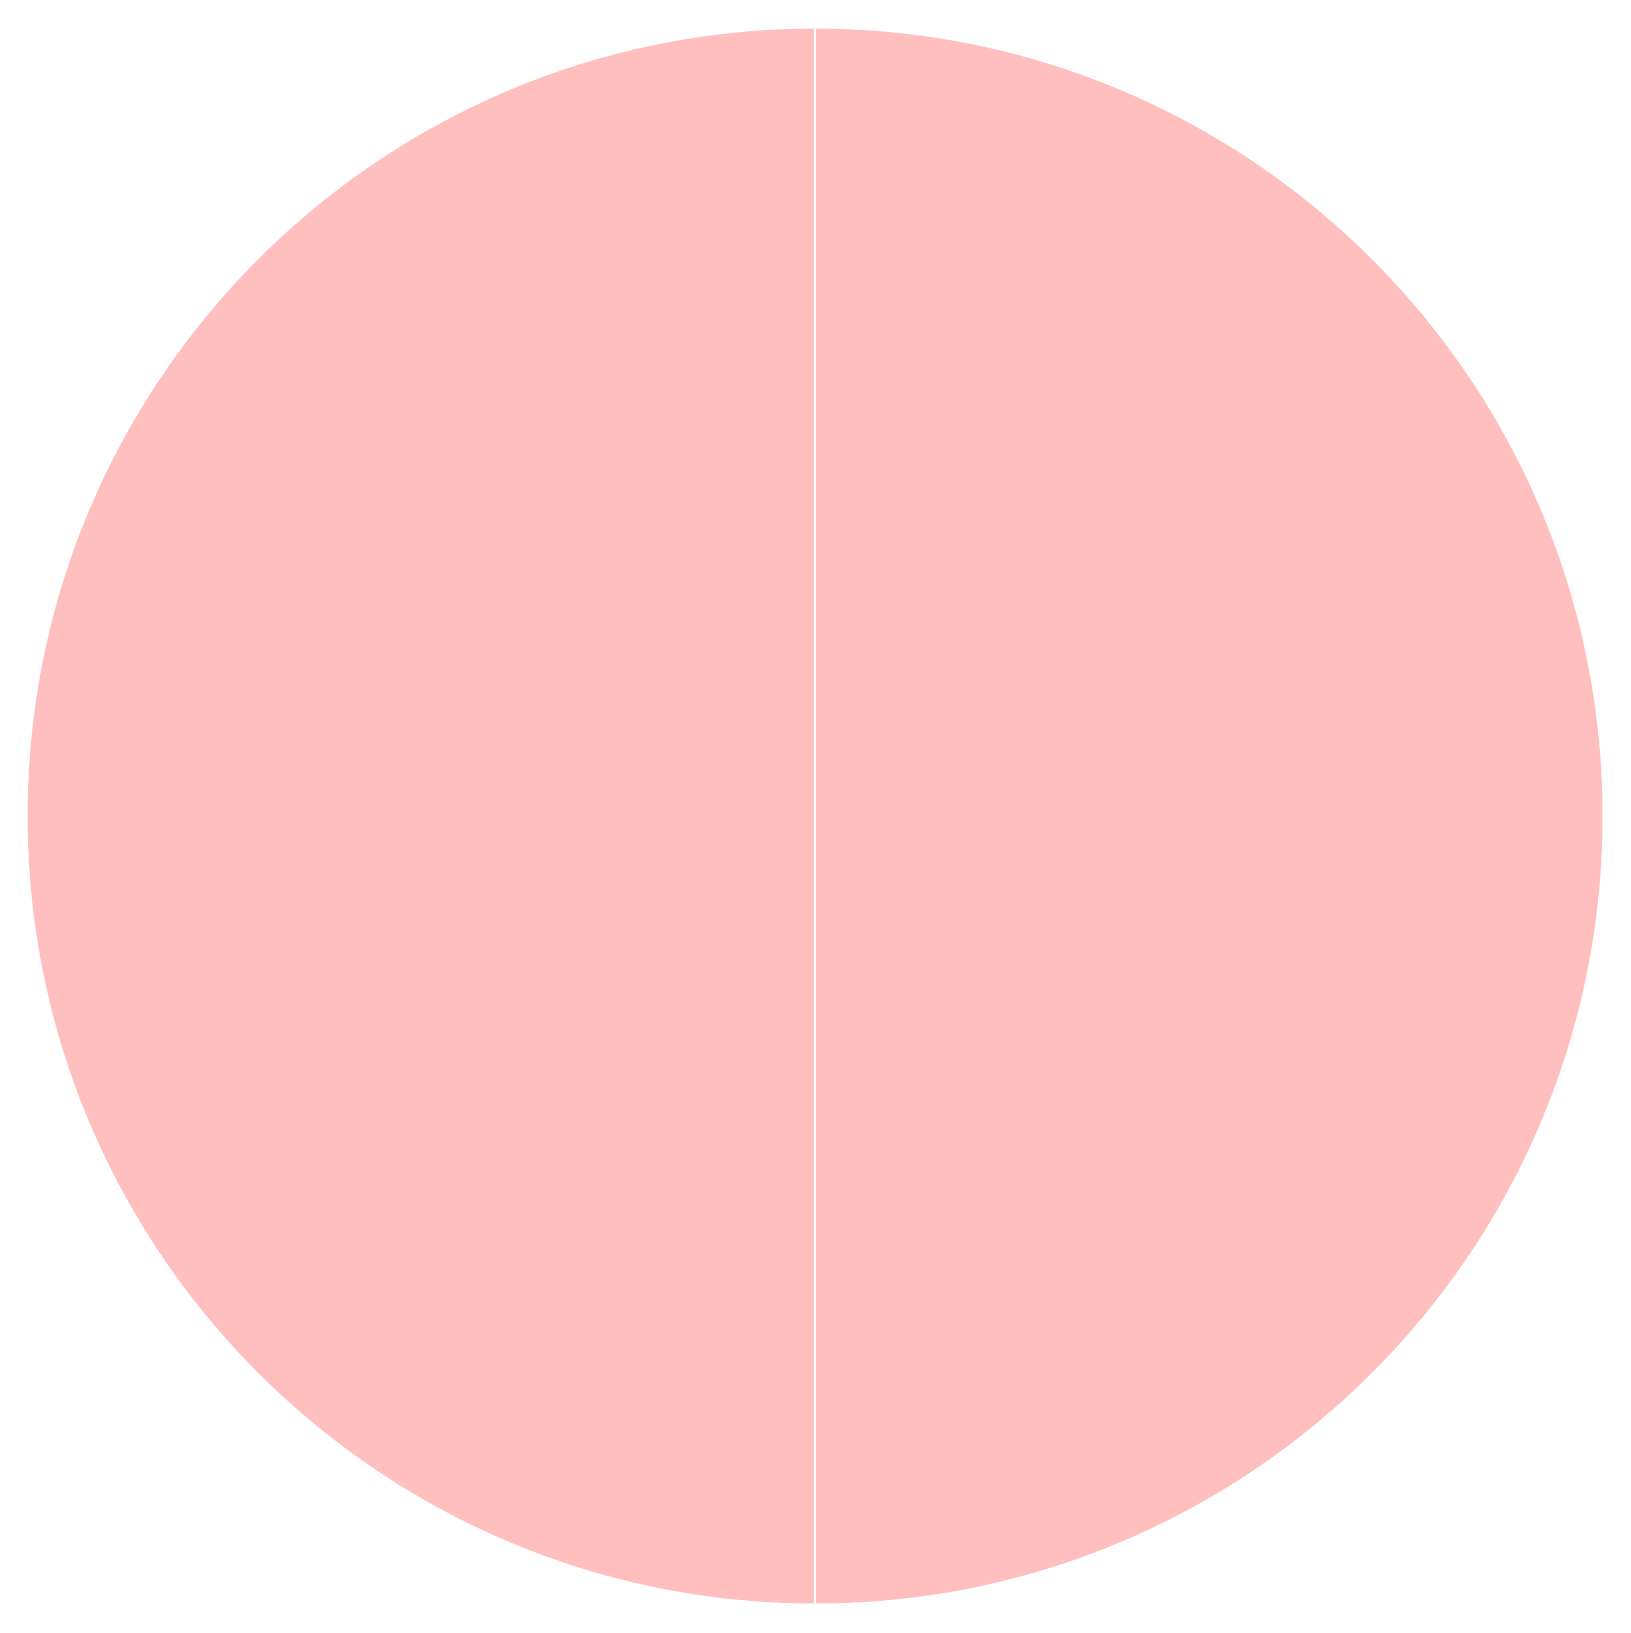
\begin{tikzpicture}
\fill[pink] (0,0) circle (10);
\draw[line width =.25mm, white] (-90:10) -- (90:10);
\end{tikzpicture}
& \quad&
 \begin{tikzpicture}
\fill[common] (0,0) circle (10);
\foreach \x in {30,150,270} \draw[line width =.25mm, white] (0,0)--(\x:10);
\end{tikzpicture}
& \quad&
 \begin{tikzpicture}
\fill[attention] (0,0) circle (10);
\foreach \x in {0,90} \draw[line width =.25mm, white] (\x:-10)--(\x:10);
\end{tikzpicture}
& \quad&
 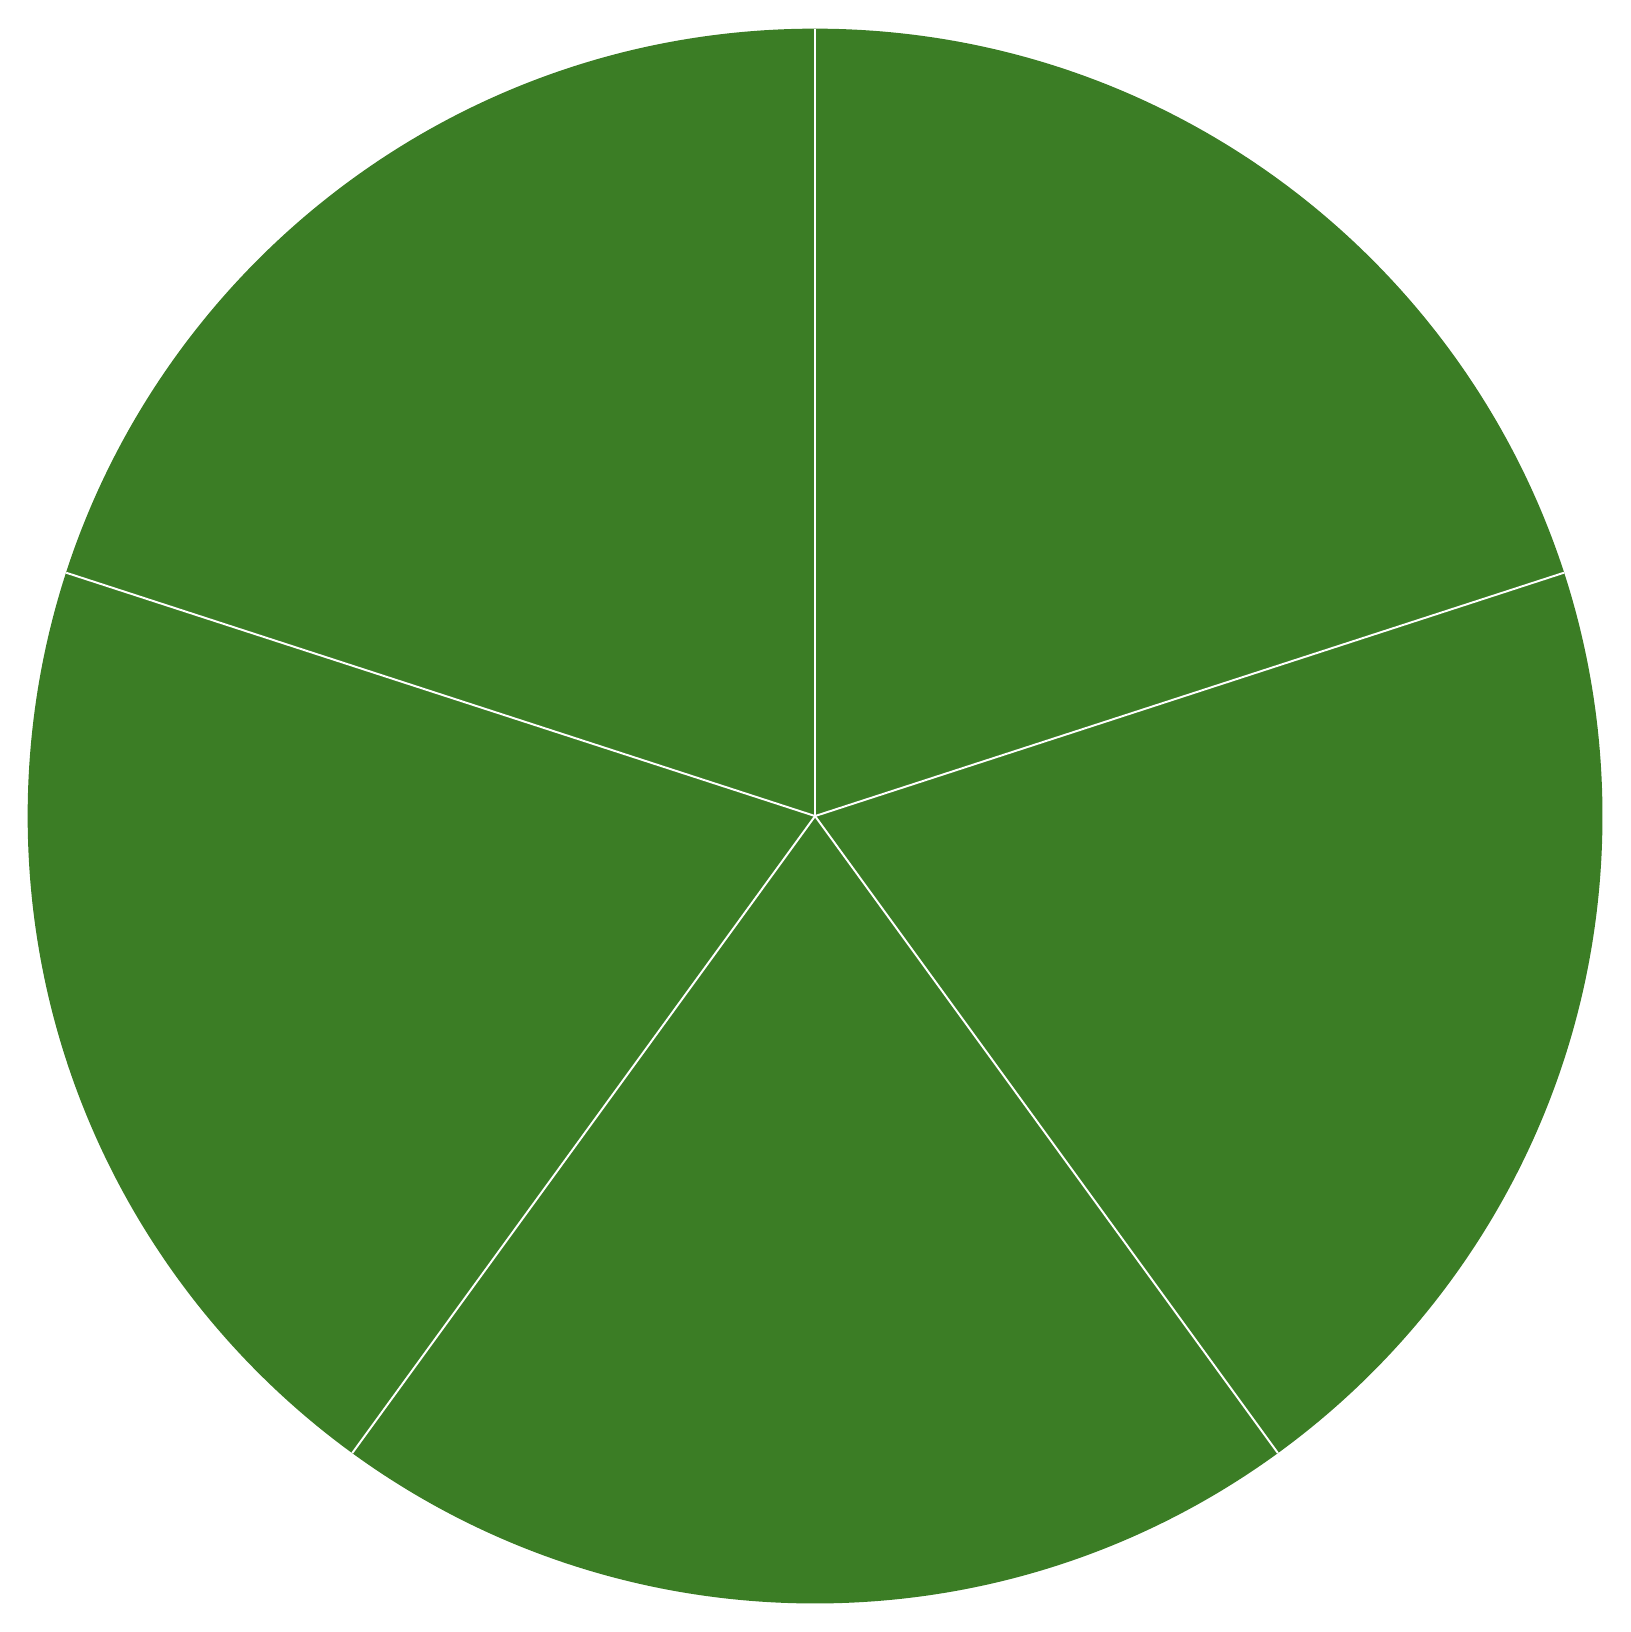
\begin{tikzpicture}
\fill[OliveGreen] (0,0) circle (10);
\foreach \x in {18,90,...,360} \draw[line width =.25mm, white] (0,0)--(\x:10);
\end{tikzpicture}\\
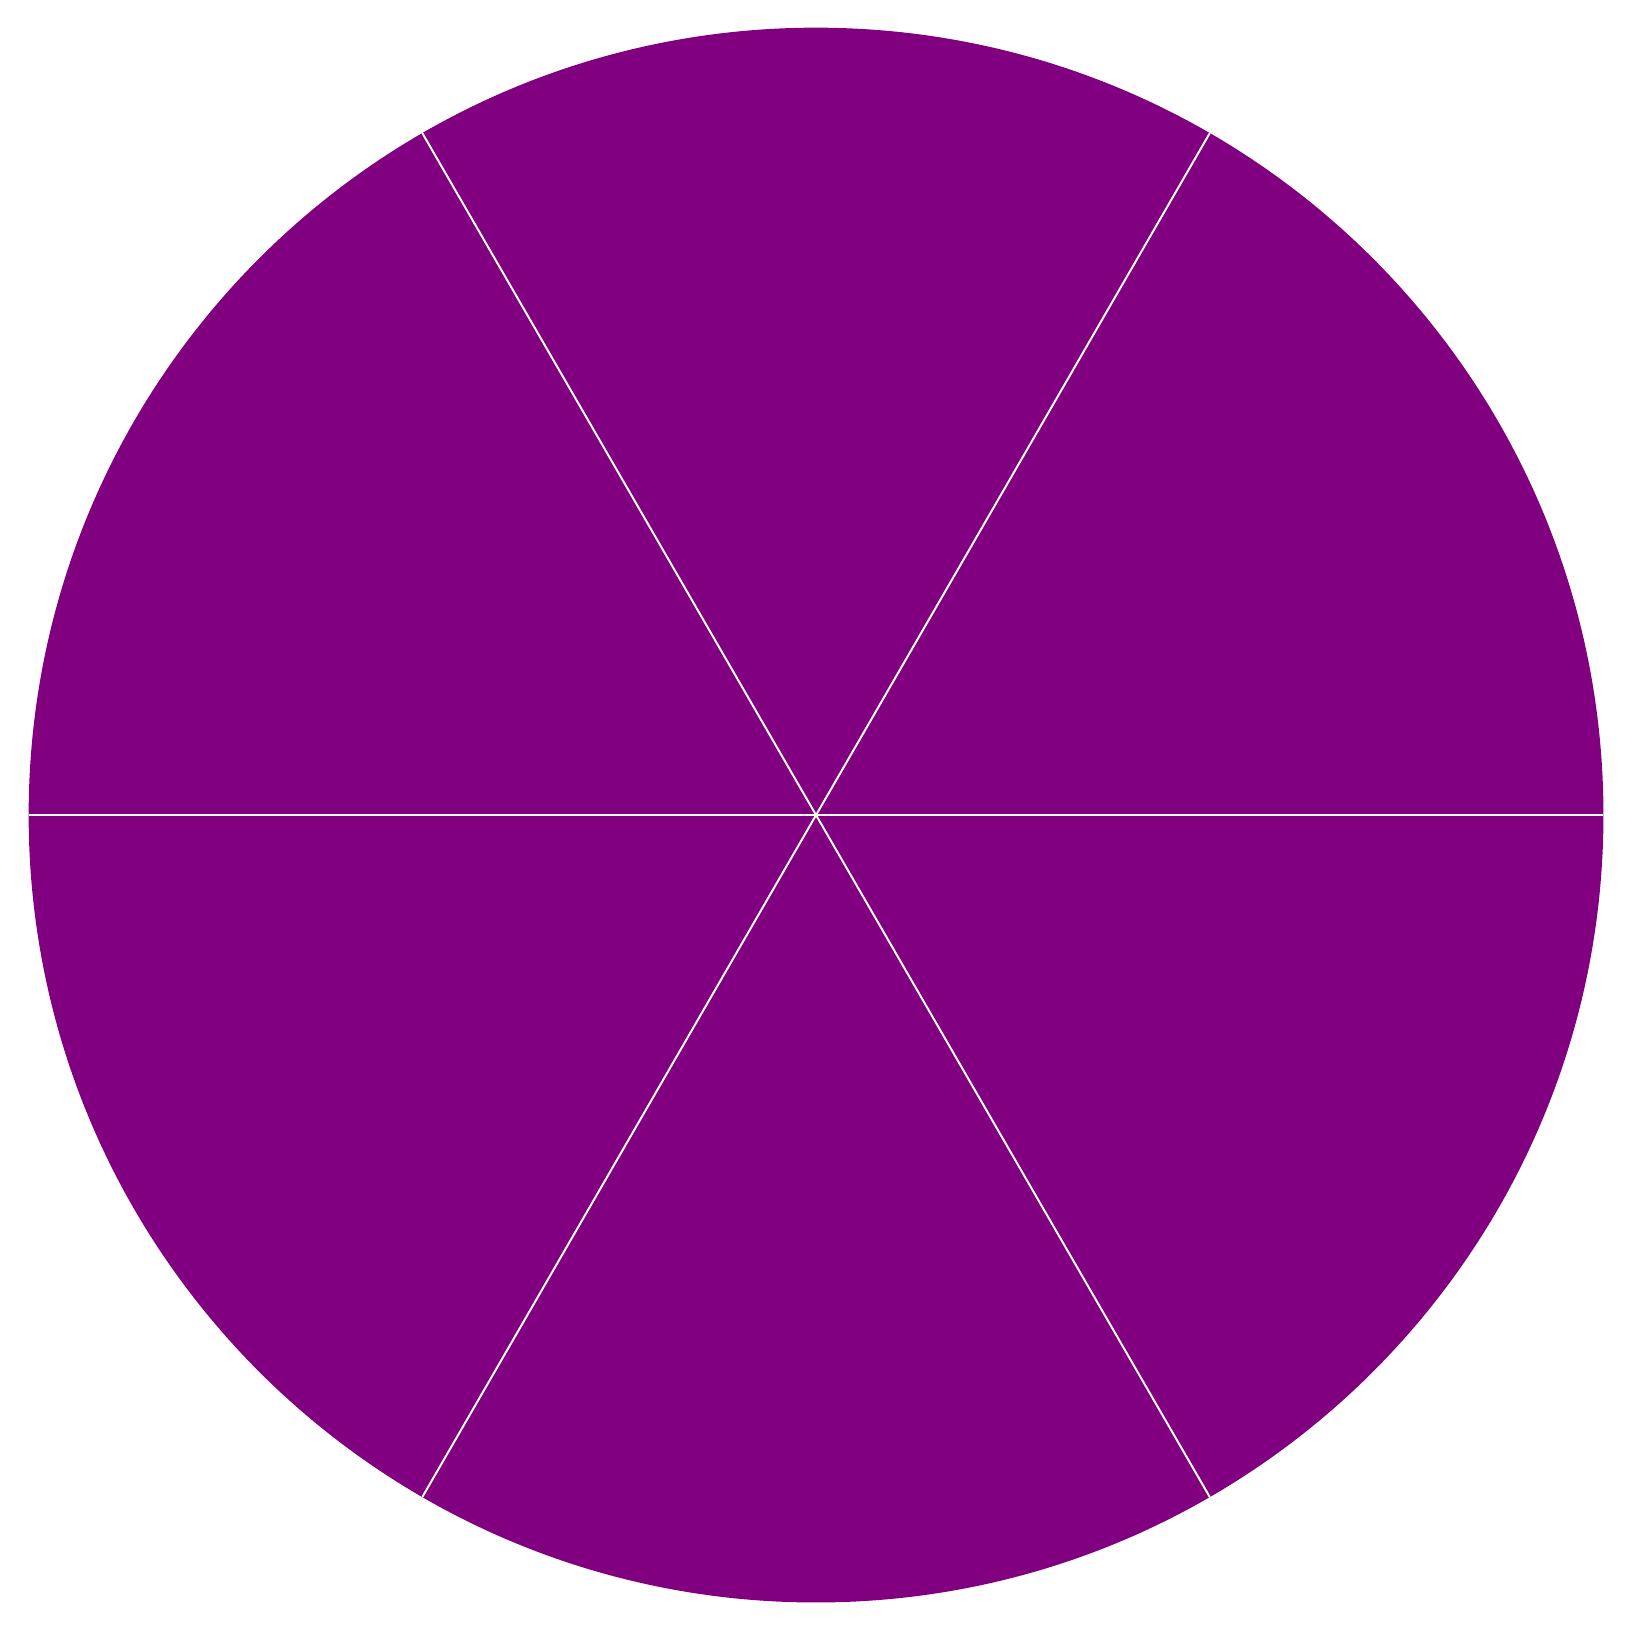
\begin{tikzpicture}
\fill[Purple] (0,0) circle (10);
\foreach \x in {0,60,...,360} \draw[line width =.25mm, white] (0,0)--(\x:10);
\end{tikzpicture}
& \parbox[t][.6cm][c]{1cm}{ }\quad&
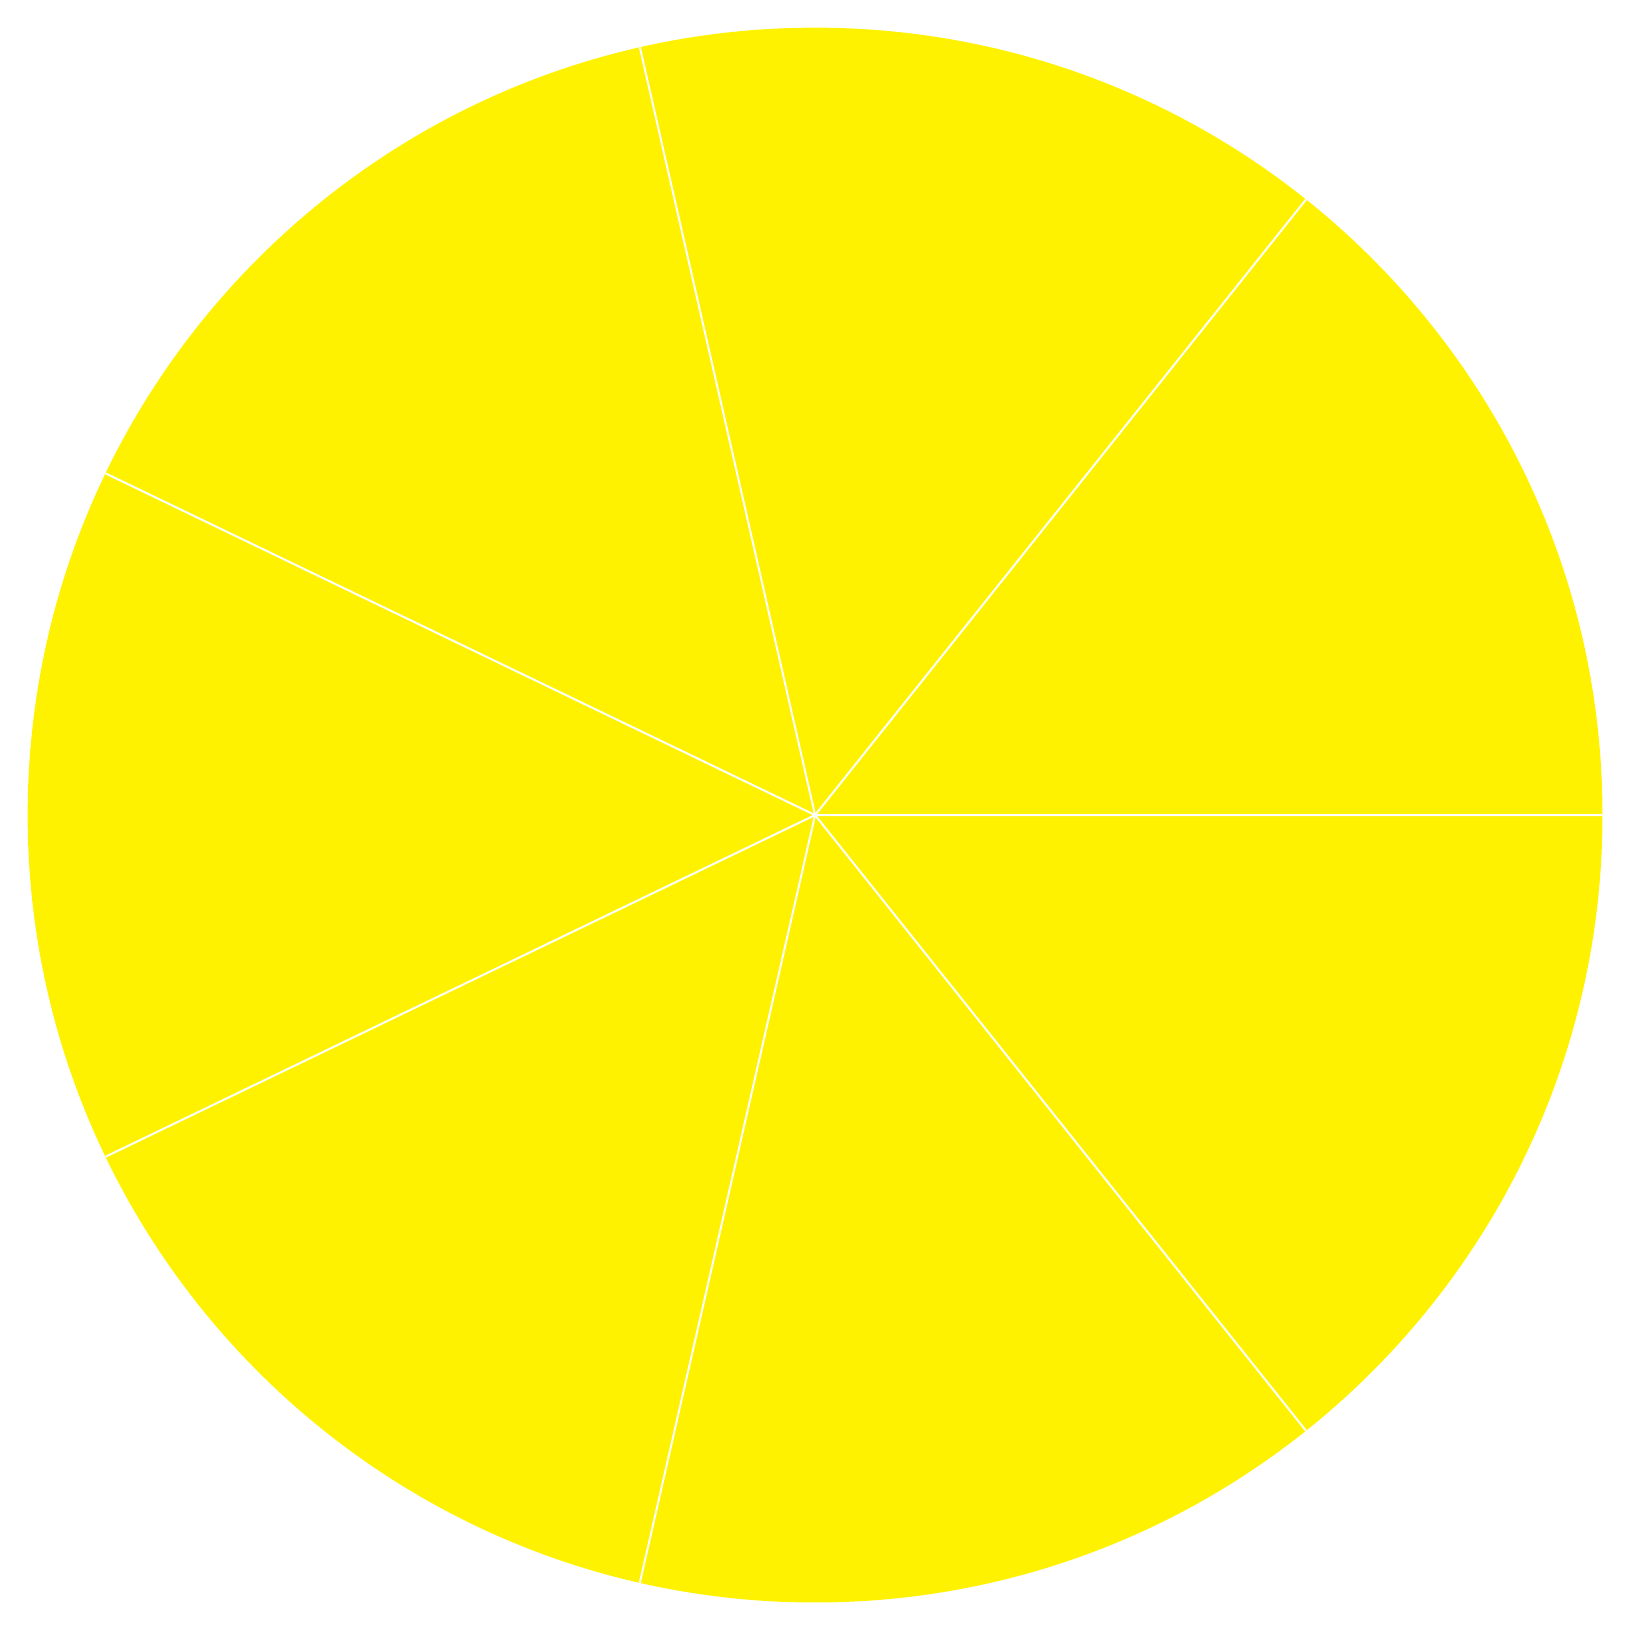
\begin{tikzpicture}
\fill[yellow] (0,0) circle (10);
\foreach \x in {0,51.428,...,360} \draw[line width =.25mm, white] (0,0)--(\x:10);
\end{tikzpicture}
&\parbox[t][.6cm][c]{1cm}{ }&
\begin{tikzpicture}
\fill[gray] (0,0) circle (10);
\foreach \x in {0,45,...,360} \draw[line width =.25mm, white] (0,0)--(\x:10);
\end{tikzpicture}
& \quad&
\begin{tikzpicture}
\fill[orange] (0,0) circle (10);
\foreach \x in {0,40,...,360} \draw[line width =.25mm, white] (0,0)--(\x:10);
\end{tikzpicture}
& \quad&
\begin{tikzpicture}
\draw (0,0) circle (10);
\foreach \x in {0,36,...,360} \draw[line width =.25mm] (0,0)--(\x:10);
\end{tikzpicture}

\end{tabular}

\end{center}

\pagebreak
\begin{enumerate}[a)]
   \item  Qual é a cor da peça que é igual a um terço do círculo preto?
  \item  Qual é a cor da peça que é igual a um quarto do círculo preto?
  \item  Qual é  a cor da peça que é igual a um sétimo do círculo preto?
  \item  Qual é a cor da peça que é igual a um nono do círculo preto?
  \item  Que fração do círculo preto é igual a uma peça de cor roxa?
  \item  Que fração do círculo preto é igual a uma peça de cor cinza?
  \item  Que fração do círculo preto é igual a uma peça de cor branca?
  \item  Que fração do círculo preto é igual a uma peça de cor rosa?
  \item  Qual fração do círculo preto é maior, um terço ou um sétimo? Explique a sua resposta.
  \item  Qual fração do círculo preto é menor, um nono ou um quarto? Explique a sua resposta.
  \item  Qual fração do círculo preto é menor, um quinto ou um sétimo? Explique a sua resposta.
  \item  Qual fração do círculo preto é maior, um oitavo ou um quarto? Explique a sua resposta.
  \item  Qual fração do círculo preto é maior, um sexto ou um sétimo? Explique a sua resposta.
\end{enumerate}

\subsection{Atividade}

Nas figuras a seguir, um mesmo círculo azul aparece diferentemente dividido em regiões iguais e colorido em vermelho.
\begin{enumerate} [\quad a)] %s
  \item     Complete as sentenças a seguir identificando os círculos que as tornam verdadeiras.
\begin{enumerate} [\quad I)] %d
      \item        	A parte do círculo  colorida em vermelho na figura \begin{tikzpicture} \draw (0,0) -- (9,0);\end{tikzpicture} é um quinto do círculo.
      \item        	A parte do círculo colorida em vermelho na figura \begin{tikzpicture} \draw (0,0) -- (9,0);\end{tikzpicture} é a sexta parte do círculo.
      \item        	A parte do círculo colorida em vermelho na figura \begin{tikzpicture} \draw (0,0) -- (9,0);\end{tikzpicture} é um sétimo do círculo.
      \item        	A parte do círculo colorida em vermelho na figura \begin{tikzpicture} \draw (0,0) -- (9,0);\end{tikzpicture} é um oitavo do círculo.
      \item        	A parte do círculo colorida em vermelho na figura \begin{tikzpicture} \draw (0,0) -- (9,0);\end{tikzpicture} é a nona parte do círculo.
      \item        	A parte do círculo colorida em vermelho na figura \begin{tikzpicture} \draw (0,0) -- (9,0);\end{tikzpicture} é um décimo do círculo.
\end{enumerate} %d

\begin{center}
\begin{tabular*}{\textwidth}{ccccc}

\begin{tikzpicture}[x=1mm,y=1mm, scale=0.5]
      \draw[fill=common, fill opacity=.3] (0,0) circle (20);
      \draw[attention,fill] (0,0)
        -- ({7 * 360/9}:20) arc ({7 * 360/9}:{8 * 360/9}:20) -- (0,0);
	  \foreach \x in {1,...,9}
    	{ \draw (0,0) -- ++({360 * \x / 9}:20); }
    	\draw (0,0) circle (20);
	  \node at (-20,16) {A)};
\end{tikzpicture}

&

\begin{tikzpicture}[x=1mm,y=1mm, scale=0.5]
      \draw[fill=common, fill opacity=.3] (0,0) circle (20);
      \draw[attention,fill] (0,0)
        -- ({3 * 360/8}:20) arc ({3 * 360/8}:{4 * 360/8}:20) -- (0,0);
	  \foreach \x in {1,...,8}
    	{ \draw (0,0) -- ++({360 * \x / 8}:20); }
    	\draw (0,0) circle (20);
	  \node at (-20,16) {B)};
\end{tikzpicture}

&
%C)

\begin{tikzpicture}[x=1mm,y=1mm, scale=0.5]
	  \draw[fill=attention] (0,0) circle (20);
	  \node at (-20,16) {C)};
\end{tikzpicture}

&
%D)
\begin{tikzpicture}[x=1mm,y=1mm, scale=0.5]
      \draw[fill=common, fill opacity=.3] (0,0) circle (20);
      \draw[attention,fill] (0,0)
        -- ({1.5 * 360/6}:20) arc ({1.5 * 360/6}:{2.5 * 360/6}:20) -- (0,0);
	  \foreach \x in {1.5,...,6.5}
    	{ \draw (0,0) -- ++({360 * \x / 6}:20); }
    	\draw (0,0) circle (20);
	  \node at (-20,16) {D)};
\end{tikzpicture}
&
%E)
\begin{tikzpicture}[x=1mm,y=1mm, scale=0.5]
      \draw[fill=common, fill opacity=.3] (0,0) circle (20);
      \draw[attention,fill] (0,0)
        -- (90 :20) arc (90:210:20) -- (0,0);
	  \foreach \x in {1,...,3}
    	{ \draw (0,0) -- ++({90 + 360 * \x / 3}:20); }
    	\draw (0,0) circle (20);
	  \node at (-20,16) {E)};
\end{tikzpicture}
\\
%F)
\begin{tikzpicture}[x=1mm,y=1mm, scale=0.5]
      \draw[fill=common, fill opacity=.3] (0,0) circle (20);
      \draw[attention,fill] (0,0)
        -- ({10 + 5 * 360/10}:20) arc ({10 + 5 * 360/10}:{10+6 * 360/10}:20) -- (0,0);
	  \foreach \x in {1,...,10}
    	{ \draw (0,0) -- ++({10 + 360 * \x / 10}:20); }
    	\draw (0,0) circle (20);
	  \node at (-20,16) {F)};
\end{tikzpicture}
&

%G)
\begin{tikzpicture}[x=1mm,y=1mm, scale=0.5]
      \draw[fill=common, fill opacity=.3] (0,0) circle (20);
      \draw[attention,fill] (0,0)-- ({90- 360/5}:20) arc ({90- 360/5}:90:20) -- (0,0);
	\foreach \x in {1,...,5}
    	{ \draw (0,0) -- ++({90 + 360 * \x / 5}:20); }
    	\draw (0,0) circle (20);
	\node at (-20,16) {G)};
\end{tikzpicture}
&
%H)
\begin{tikzpicture}[x=1mm,y=1mm, scale=0.5]
  \draw[attention,fill] (0,0)-- (90:20) arc (90:-90:20) -- (0,0);
  \draw (0,0)-- (90:20) arc (90:-90:20) -- (0,0) --cycle;
  \draw[fill=common, fill opacity=.3] (0,0)-- (90:20) arc (90:270:20) -- (0,0) -- cycle;
  \draw (0,0) circle (20);
  \node at (-20,16) {H)};
\end{tikzpicture}
&
%I)
\begin{tikzpicture}[x=1mm,y=1mm, scale=0.5]
      \draw[fill=common, fill opacity=.3] (0,0) circle (20);
      \draw[attention,fill] (0,0)-- ({- 360/7}:20) arc ({- 360/7}:{-2 * 360/7}:20) -- (0,0);
	  \foreach \x in {1,...,7}
    	{ \draw (0,0) -- ++({360 * \x / 7}:20); }
    	\draw (0,0) circle (20);
	  \node at (-20,16) {I)};
\end{tikzpicture}
&
%J)
\begin{tikzpicture}[x=1mm,y=1mm, scale=0.5]
      \draw[fill=common, fill opacity=.3] (0,0) circle (20);
      \draw[attention,fill] (0,0)-- (0:20) arc (0:{- 360/4}:20) -- (0,0);
	  \foreach \x in {1,...,4}
    	{ \draw (0,0) -- ++({360 * \x / 4}:20); }
    	\draw (0,0) circle (20);
	  \node at (-20,16) {J)};
\end{tikzpicture}

 \end{tabular*}
\end{center}

  \item     Dentre as frações do círculo destacadas em vermelho, identifique uma que seja menor do que um sexto do círculo.
  \item     Dentre as frações do círculo destacadas em vermelho, identifique uma que seja maior do que um nono do círculo.
  \item     Identifique uma fração do círculo que seja menor do que um sexto e maior do que um nono do círculo.
\end{enumerate} %s

\pagebreak
\subsection{Atividade}

Em cada uma das imagens, a parte em vermelho é uma fração da figura. Essas frações podem ser ``um meio'', ``um quarto'' ou ``um décimo'' da figura. Associe cada imagem à fração correspondente.

\begin{center}
\begin{tabular*}{\textwidth}{m{0.3\textwidth}m{0.3\textwidth}m{0.3\textwidth}}
a)
\parbox[t][2cm][c]{2cm}{
\begin{tikzpicture}[scale=5]
 \draw[fill=common, fill opacity=.3] (0,0) rectangle (4,2);
 \filldraw[fill=attention, draw=black] (0,0) -- (4,2) -- (4,0) -- cycle;
\end{tikzpicture}}
&
b)
\parbox[t][2cm][c]{2cm}{
\begin{tikzpicture}[scale=5]
 \draw[fill=common, fill opacity=.3] (0,0) rectangle (4,2);
 \foreach \n in {0.4,0.8,1.2,...,3.2,3.6}{
 \draw (\n,0) -- (\n,2);}
 \filldraw[fill=attention, draw=black] (0.8,0) -- (0.8,2) -- (1.2,2) -- (1.2,0) -- cycle;
\end{tikzpicture}}
&
c)
\parbox[t][2cm][c]{2cm}{
\begin{tikzpicture}[scale=5]
 \draw[fill=common, fill opacity=.3] (0,0) rectangle (4,2);
 \filldraw[fill=attention, draw=black] (2,1) rectangle (4,2);
 \draw (0,1) -- (4,1);
 \draw (2,0) -- (2,2);
 \end{tikzpicture}}
\\

d)
\parbox[t][2cm][c]{2cm}{
\begin{tikzpicture}[scale=5]
 \draw[fill=common, fill opacity=.3] (135:2) arc (135:405:2) -- (0,0) --cycle;
 \filldraw[fill=attention, draw=black] (45:2) arc (45:135:2) -- (0,0) -- cycle;
 \end{tikzpicture}}
&
e)
\parbox[t][2cm][c]{2cm}{
\begin{tikzpicture}[scale=5]
 \draw[fill=common, fill opacity=.3] (0:2) -- (60:2) -- (90:1.73) -- (0,0) -- (180:2) -- (240:2) -- (300:2) --cycle;
 \filldraw[fill=attention, draw=black] (-2,0) -- (0,0) -- (0,1.73) -- (120:2) -- cycle;
\end{tikzpicture}}
&
f)
\parbox[t][2cm][c]{2cm}{
\begin{tikzpicture}[scale=5]
 \draw[fill=common, fill opacity=.3] (0,0) rectangle (5,1);
 \draw[fill=attention] (0,1) rectangle (5,2);
\end{tikzpicture}}
\\
g)
\parbox[t][2cm][c]{2cm}{
\begin{tikzpicture}[scale=5]
 \draw[fill=common, fill opacity=.3] (0,.75) rectangle (2,3);
 \draw[fill=attention] (0,0) rectangle (2,.75);
\end{tikzpicture} }
 &
h)
\parbox[t][2cm][c]{2cm}{
\begin{tikzpicture}[scale=5]
 \draw[fill=common, fill opacity=.3] (236:2) arc (236:560:2);
 \draw[fill=attention] (200:2) arc (200:236:2) -- (0,0) -- cycle;
\end{tikzpicture} }
&
i)
\parbox[t][2cm][c]{2cm}{
\begin{tikzpicture}[scale=5]
 \draw[ultra thick,color=attention] (-1,0) arc (180:270:1);
 \draw (0,-1) arc (270:360:1) -- (1,0) arc (180:0:1);
 \end{tikzpicture}}
\\
j)
\parbox[t][2cm][c]{2cm}{

\begin{tikzpicture}
\tikzset{
  annotated cuboid/.pic={
    \tikzset{%
      every edge quotes/.append style={midway, auto},
      /cuboid/.cd,
      #1
    }
    \draw [every edge/.append style={pic actions, densely dashed, opacity=0}, pic actions]
    (0,0,0) coordinate (o) -- ++(-\cubescale*\cubex,0,0) coordinate (a) -- ++(0,-\cubescale*\cubey,0) coordinate (b) edge coordinate [pos=1] (g) ++(0,0,-\cubescale*\cubez)  -- ++(\cubescale*\cubex,0,0) coordinate (c) -- cycle
    (o) -- ++(0,0,-\cubescale*\cubez) coordinate (d) -- ++(0,-\cubescale*\cubey,0) coordinate (e) edge (g) -- (c) -- cycle
    (o) -- (a) -- ++(0,0,-\cubescale*\cubez) coordinate (f) edge (g) -- (d) -- cycle;
 },
  /cuboid/.search also={/tikz},
  /cuboid/.cd,
  width/.store in=\cubex,
  height/.store in=\cubey,
  depth/.store in=\cubez,
  units/.store in=\cubeunits,
  scale/.store in=\cubescale,
  width=100,
  height=100,
  depth=100,
  units=cm,
  scale=.1,
}
    \draw[dotted] (2.95,-1.9) -- (25.5,-1.9);
    \pic [fill=attention, fill opacity=.8] at (0,0) {annotated cuboid={width=25, height=50, depth=8}};
    \pic [fill=common, fill opacity=.3] at (22.5,0) {annotated cuboid={width=225, height=50, depth=8}};
\end{tikzpicture}}
&

l)
\parbox[t][2cm][c]{2cm}{
\begin{tikzpicture}[scale=5]
 \draw[fill=attention] (0,2) rectangle (2,4);
 \draw[fill=common, fill opacity=.3] (0,0) rectangle (2,2);
 \draw[fill=common, fill opacity=.3] (2,0) rectangle (4,2);
 \draw[fill=common, fill opacity=.3] (2,2) rectangle (4,4);
 \end{tikzpicture} }
&
m)
\parbox[t][2cm][c]{2cm}{
\begin{tikzpicture}[scale=5]
\draw[fill=common, fill opacity=.3] (0,0) rectangle (4,4);
 \filldraw[fill=attention, draw=black] (1,0) rectangle (2,1);
 \filldraw[fill=attention, draw=black] (3,0) rectangle (4,1);
 \filldraw[fill=attention, draw=black] (0,1) rectangle (1,2);
 \filldraw[fill=attention, draw=black] (2,1) rectangle (3,2);
 \filldraw[fill=attention, draw=black] (1,2) rectangle (2,3);
 \filldraw[fill=attention, draw=black] (3,2) rectangle (4,3);
 \filldraw[fill=attention, draw=black] (0,3) rectangle (1,4);
 \filldraw[fill=attention, draw=black] (2,3) rectangle (3,4);
\end{tikzpicture}}

\end{tabular*}
\end{center}
